\chapter{GeV-Scale LFV Axion-Like Particles in Collider Experiments}
\label{alp_collider}


\vspace{-1cm}
\begin{center}
{\it This chapter is based on work done in Refs.~\cite{Davoudiasl:2021haa,Davoudiasl:2021mjy,Davoudiasl:2024vje,Batell:2024cdl}.}
\end{center}
\vspace{1cm}


\section{Introduction}

One of the biggest potential challenges for discovery in modern-day particle physics is the vast disparity of scales between our current highest energy experiments (${\cal O}(10^4~{\rm GeV})$), and the Planck scale ($10^{18}~{\rm GeV}$). In principle, new physics can lie anywhere between these two scales, possibly far beyond the reach of our experimental capabilities. A naive estimate for the scale that generates neutrino mass yields $\Lambda \sim 10^{15}~{\rm GeV}$, which is intriguingly close to the expected scale of grand unification \cite{Mohapatra:2004fj}. If new physics doesn't appear until this scale (or even many orders of magnitude below it), how can we ever hope to make progress in the field?

Axion-like particles (ALPs) offer a promising way out of this conundrum. As described in Section \ref{sec:ALP}, ALPs are the pseudo-Nambu-Goldstone bosons of spontaneously broken approximate global symmetries. By virtue of this definition, they are light relative to the physics scale from whence they came. While the discovery of an ALP wouldn't give us a complete description of the underlying physics, analyzing its couplings to the SM particles would help us determine the symmetry-breaking scale, potentially guiding design for future particle-physics experiments. 

ALPs are often thought of as very light, but they can generically be quite heavy if their associated global symmetry is spontaneously broken at a large scale or if the explicit breaking of said symmetry is substantial. In Chapter 2, we encountered a few scenarios in which the low-energy effective theory contained ALPs with multi-GeV masses, namely ALPs from ${\Bbb Z}_N$ Froggatt-Nielsen models \cite{Greljo:2024evt} and dark pions from composite dark matter models \cite{Davoudiasl:2017zws}. The prospect of new particles at this scale which couple to the SM is exciting, as they are in a ``Goldilocks zone'' for modern experiments: not so heavy that they can't be produced in GeV or TeV-scale collisions, but not so light that they decay far beyond the confines of the experimental apparatus. In addition to lying within an accessible mass range, the ALPs in these models also exhibit LFV couplings to the ALP, offering an enticing avenue for their discovery. While we have only focused on a few scenarios in which LFV ALPs arise, we note that any UV theory that couples to the lepton sector of the SM will contain LFV unless it is explicitly protected.

We have already explored limits on LFV couplings to the ALPs in Chapter 2. Notably, the limits become much weaker for $m_a > m_\tau$, since the heavily constrained decay mode $\tau \rightarrow \ell_i\ell_j\bar{\ell}_k$ can no longer proceed via an on-shell ALP. In this regime, Fig.~\ref{fig:LFV_limits} indicates that a scale of $\Lambda \sim 10~{\rm TeV}$ is still very much in reach as the source of such particles. One important caveat from these limits is that they are limits on the products of two couplings. In the reasonable scenario that the on-diagonal couplings are larger than the off-diagonal couplings, one could even expect unconstrained LFV physics at $\Lambda \sim 1~{\rm TeV}$. While the leptonic decay modes involve products of the couplings, individual couplings (flavor-conserving and flavor-violating) can be probed by measurements of the lepton dipole moments. If one takes these as constraints, we have also found  $\Lambda \sim 1~{\rm TeV}$. 

Given their direct coupling to leptons, one might expect strong limits for such ALPs to come from electron-positron colliders such as LEP and CESR via the production-process $e^+ e^- \rightarrow a \gamma$ or the $s$-channel $e^+ e^- \rightarrow a^*\rightarrow \ell^+ \ell'^-$. However, due to the mass-dependence of ALP-fermion couplings, the cross-section of this process would be suppressed by $m_e^2/\Lambda^2 \sim 10^{-13}$ for $\Lambda = 1~{\rm TeV}$. Hence, we are forced to look elsewhere for signatures of such particles. 

In the event that the LFV ALP couples to the Higgs (as is the case for the composite ALP from Ref.~\cite{Davoudiasl:2017zws}), one promising avenue for discovery is through decays of the form $h \rightarrow a a \rightarrow \ell^+\ell'^-\ell^+\ell'^-$ for $\ell \neq \ell'$, as this is a very distinct LFV final-state. LFV decays of the Higgs boson of this form were studied previously in Ref.~\cite{Evans:2019xer}, but in that work the intermediate particles were taken to be scalar rather than ALPs. With ALPs, the parameter space of constraints will be somewhat different. In particular, since the ALP decay widths are proportional to the mass-squared of the final-state particles, decays of the form $h \rightarrow aa \rightarrow \tau^\pm\tau^\pm \ell^\mp \ell'^\mp$ will be dominant.

An alternative approach which does not rely on a Higgs coupling is production from coherent electromagnetic interactions between leptons and heavy nuclei ($\ell^- A_Z \rightarrow \ell^- A_Z a$), such as those studied in Chapter 4. While most existing electron and muon beam dumps have energies too small to produce GeV-scale ALPs at any appreciable rate, this may change with research and development into a multi-TeV muon collider \cite{Delahaye:2013jla,Long:2020wfp,Accettura:2023ked}. In addition, the Electron Ion Collider (EIC) will be the equivalent of a multi-TeV electron beam dump in the rest frame of the heavy nuclei,\footnote{With a sacrifice in luminosity.} so peripheral production of GeV-scale particles will be possible. Looking forward, the case has been made for a future Muon (Synchrotron)-Ion Collider (MuSIC) due to its potential to probe nuclear substructure \cite{Acosta:2021qpx,Acosta:2022ejc} and new physics beyond the SM \cite{Davoudiasl:2024vje}. The benefit of these approaches is that, up to the branching of the final-state ALP, they are independent from the other couplings in the model. Hence, they provide an absolute constraint on the coupling $C_{\tau \ell}/\Lambda$. 

In this Chapter, we will explore constraints on GeV-scale LFV ALPs in various collider settings. In Section \ref{sec:higgs_decay}, we find limits on such particles at the LHC in the presence of a Higgs portal interaction for the ALP. In  Section \ref{sec:EIC_ALP}, we examine limits on the $e\tau$ coupling of the ALP from the upcoming EIC, and explore a region of the parameter space for which the interaction can explain either of the electron $g-2$ anomalies. In Section \ref{sec:MuBeD_MuSIC_ALP}, we repeat this analysis for a muon beam dump experiment (MuBeD) along with the hypothetical MuSIC experiment, exploring a region of the $\mu\tau$ coupling parameter space that is of interest for the muon $g-2$ anomaly.

\section{Higgs Decays at the LHC}\label{sec:higgs_decay}

We begin by studying LFV ALPs with a significant Higgs-portal interaction, under the assumption that the ALP is leptophilic. Then, the relevant terms from the EFT Lagrangian \ref{eq:ALP_EFT} are \cite{Georgi:1986df,Bauer:2020jbp}
\begin{align}
    {\cal L} &= \frac{1}{2}(\partial_\mu a)^2 - \frac{1}{2}m_a^2 a^2 + {\cal L}_{\ell} + {\cal L}_h \\
\intertext{where the ALP-lepton interaction is given by}
    {\cal L}_\ell &= \frac{\partial_\mu a}{\Lambda} \sum_{\ell, \ell'}\bar{\ell}\gamma^\mu[A_{\ell\ell'} - \gamma_5 V_{\ell \ell'}]\ell' + {\rm H.c.}
\intertext{and the ALP-Higgs interaction is }
    {\cal L}_h &= \frac{C_{ah}}{\Lambda} v (\partial_\mu a)^2 h + \frac{C_{ah}'}{\Lambda^2}vm_a^2a^2 h. \label{eq:ALP_Higgs_int}
\end{align}
The presence and size of each coupling $C_{ah}$ and $C_{ah}'$ is dependent on the nature of the UV theory that gives rise to the ALP. Given the interaction term (\ref{eq:ALP_Higgs_int}), the decay rate for $h\rightarrow aa$ is given by
\begin{align}
    \Gamma(h\rightarrow aa) &= \frac{1}{32\pi}\frac{v^2m_h^3}{\Lambda^4}\sqrt{1-\frac{4m_a^2}{m_h^2}}\left(C_{ah}-2(C_{ah}-C_{ah}')\frac{m_a^2}{m_h^2}\right)^2.
\end{align}
At this point, it is useful to parametrize the Higgs decay rate in terms of an effective ALP-Higgs coupling:
\begin{align}
    \Gamma(h\rightarrow aa) &= \frac{1}{32\pi}\frac{v^2m_h^2}{\Lambda^4}\left(1-\frac{2m_a^2}{m_h^2}\right)^2\sqrt{1-\frac{4m_a^2}{m_h^2}}\overline{C}_{ah}^2
\end{align}
where
\begin{align}
    \overline{C}_{ah} &\equiv C_{ah} + C_{ah}'\frac{2m_a^2}{m_h^2-2m_a^2}.
\end{align}
Rather than presenting limits on $C_{ah}$ and $C_{ah}'$ independently, we will focus on limits on the combined effective coupling $\overline{C}_{ah}$ for the majority of this section. We will specialize to certain values of $C_{ah}$ and $C_{ah}'$ in Section \ref{sec:higgs_combined}.

For $m_a > m_\ell + m_{\ell'}$, the process $a \rightarrow \ell \ell'$ occurs with decay width
\begin{align}
    \Gamma(a \rightarrow \ell\ell') &= \frac{C_{\ell\ell'}^2}{8\pi \Lambda^2}\left[m_{\ell\ell'}^2(\Theta_{\ell\ell'}) - \frac{(m_\ell^2-m_{\ell'}^2)^2}{m_a^2}\right]\sqrt{\left(m_a^2-(m_\ell-m_{\ell'})^2\right)\left(m_a^2-(m_\ell+m_{\ell'})^2\right)}
\end{align}
where $C_{\ell\ell'} = \sqrt{|A_{\ell \ell'}|^2 + |V_{\ell \ell'}|^2}$, $\Theta_{\ell\ell'} = \tan^{-1}\left|V_{\ell\ell'}/A_{\ell\ell'}\right|$, and $m_{\ell\ell'}^2(\Theta) = m_\ell^2 + m_{\ell'}^2 + 2m_\ell m_{\ell'}\cos{2\Theta}$. Due to the lepton mass hierarchy, either $m_{\ell'} = m_\ell$ or (without loss of generality) $m_{\ell'} \ll m_\ell$, so it is useful to express the width in each of these cases: 
\begin{align}
    \Gamma(a \rightarrow \ell^\pm \ell'^\mp) &= \frac{m_a}{8\pi}\frac{m_\ell^2}{\Lambda^2}\begin{cases}  \ \,C_{\ell\ell'}^2(1 - m_{\ell}^2/m_a^2)^2& \ell' \ll \ell,\\
    4A_{\ell\ell}^2(1 - 4m_\ell^2/m_a^2)^{1/2} & \ell' = \ell.
    \end{cases}
\end{align}
Notably, the decay rate is proportional to the square of the heavier lepton mass, so the ALP will almost always decay via $a\rightarrow \tau \ell$. For equivalent couplings and $m_a \gg m_\ell \gg m_{\ell'}$, we have $\Gamma(a\rightarrow \ell \ell)\approx 4\Gamma(a\rightarrow \ell \ell')$. Hence, one expects the dominant decay mode of the ALP to be $a\rightarrow \tau\tau$, followed by $a \rightarrow \tau \ell$ with $\ell = e$ or $\mu$. Of course, this is subject to change based on the underlying hierarchies between the ALP-lepton couplings.

Even in the absence of a photon coupling, the $a\rightarrow \gamma\gamma$ decay mode is generated at loop level via a triangle diagram. Specializing  Eq.~\ref{eq:Cgg_eff} to the case of only leptonic couplings, we have
\begin{align}
    \Gamma(a\rightarrow \gamma\gamma) &= \frac{4\pi \alpha^2 m_a^3}{\Lambda^2}|C_{\gamma\gamma}^{\rm eff.}|^2,\\
\intertext{where}
    C_{\gamma\gamma}^{\rm eff.} &= \sum_{\ell}\frac{A_{\ell\ell}}{8\pi^2}B_1(4m_\ell^2/m_a^2)
\end{align}
\begin{figure}[t!]
    \centering
    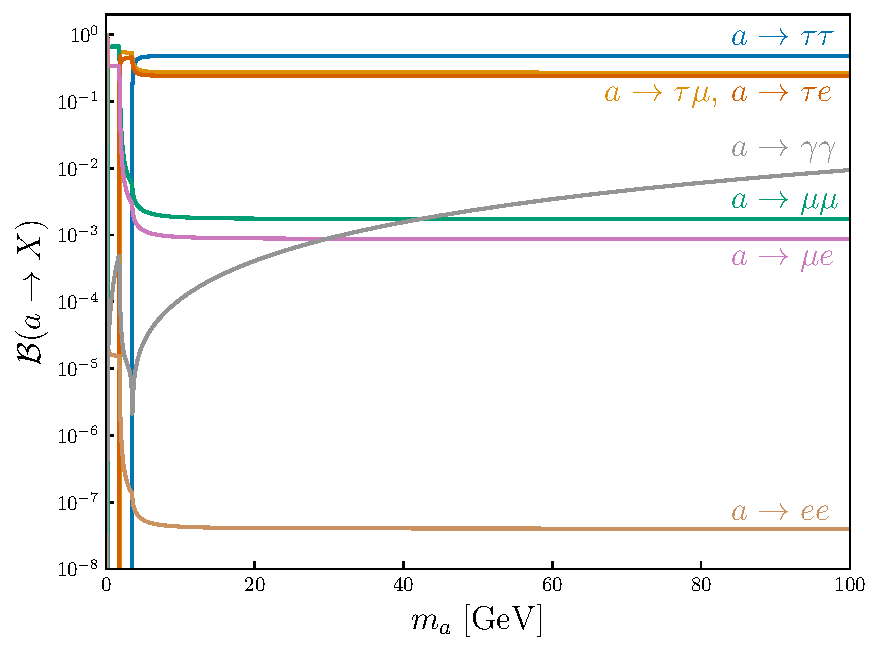
\includegraphics[width=0.7\linewidth]{figures/chapter5/LFV_ALP_branching_fraction.pdf}
    \caption[ALP branching fraction assuming a democratic lepton coupling matrix.]{ALP branching fraction assuming a democratic lepton coupling matrix (and all other couplings zero). The ALP will decay to at least one $\tau$ roughly $99.7\%$ of the time.}
    \label{fig:LFV_ALP_branching_fraction}
\end{figure}
and $B_1$ is given in Eq.~\ref{eq:B1}. In particular, $B_1(\tau \rightarrow 0)\rightarrow 1$, so the loop-induced photonic decay rate can grow quite large for heavy ALPs. It is worthwhile to compare the loop-induced photon decay rate to the flavor-violating decay rate $a \rightarrow \tau \ell$. Their ratio is given by
\begin{align}
\frac{\Gamma(a\rightarrow\gamma\gamma)}{\Gamma(a\rightarrow\tau^\pm\ell^\mp)} \sim  \frac{9\alpha^2}{2\pi^2}\frac{m_a^2}{m_\tau^2}\frac{|\overline{A_{\ell\ell}}|^2}{|C_{\tau \ell}|^2} \sim \left(\frac{1}{200}\frac{m_a}{m_\tau}\frac{|\overline{A_{\ell\ell}}|}{|C_{\tau\ell}|}\right)^2
\end{align}
where $\overline{A_{\ell\ell}}$ is the average of the ALP couplings to the lepton axial vector current. Hence, we see that the $a\rightarrow \gamma\gamma$ rate will become comparable to the $a\rightarrow \tau \ell$ rate when $|C_{\tau \ell}| \lesssim \frac{m_a}{200m_\tau}|\overline{A_{\ell\ell}}| $. Given that we are considering ALPs in the GeV range, it is safe to ignore this decay mode in our discussions. To emphasize this point, we plot the branching-fraction of the ALP assuming a democratic ALP-lepton coupling matrix in Fig.~\ref{fig:LFV_ALP_branching_fraction}.

For the remainder of this section, we will present limits on the model under the assumption of democratic couplings (or at the very least, $C_{\tau e}\sim C_{\tau \mu}\sim C_{\tau\tau}$). However, we should note that our results are more-or-less insensitive to this choice, because $a \rightarrow \tau \tau$ (which is always dominant) can mimic the $a \rightarrow \tau \ell$ decay mode via a leptonic decay of one of the final-state $\tau$. 

\subsection{Prompt ALP Decays at CMS}\label{sec:higgs_decay_CMS}
We will begin by considering the scenario where the ALPs are produced in Higgs decays then themselves decay promptly within the CMS detector at the LHC. We present constraints on the leptonic couplings based on the search in Ref.~\cite{CMS:2019lwf} for proton-proton collisions which result in four charged lepton final states. The Higgs decays that we are most interested in are those of the form $h \rightarrow (\tau^\pm  \ell^\mp)(\tau^\pm \ell^\mp)$ due to the strongly LFV final-state; these primarily contribute to the ``OSSF0'' signal in Ref.~\cite{CMS:2019lwf}, which corresponds to those events for which the number of opposite-sign, same-flavor (OSSF) lepton pairs is zero. The study only includes electrons and muons in the OSSF0 signal, so this requires each $\tau$ in our final-state to decay leptonically, resulting in decay modes of the form $h\rightarrow aa \rightarrow \mu^\pm \mu^\pm e^\mp e^\mp (+ {\rm neutrinos})$.

To recast this study for our model, we reproduce the LFV ALP EFT in \verb|FeynRules| \cite{Alloul:2013bka} and simulate parton-level events with \verb|MadGraph5_aMC@NLO| \cite{Alwall:2011uj}. We then use $\verb|PYTHIA8|$ for showering and simulate the CMS detector with $\verb|DELPHES|$ \cite{deFavereau:2013fsa}. We produce 50\,000 events of the form $gg\rightarrow h, h \rightarrow aa \rightarrow \rm OSSF0$ for the masses $m_a = 2$-$3.6~{\rm GeV}$ with a step of $0.2~{\rm GeV}$, and $m_a = 5$-$60~{\rm GeV}$ with a step of $5~{\rm GeV}$. We additionally consider $m_a \approx m_h/2 = 62.5~{\rm GeV}$ for a total of 22 different masses. The number of OSSF0 signal events recorded from the initial 50\,000 (along with the corresponding signal efficiency$\cdot$ acceptance), based on the analysis conducted in Ref.~\cite{CMS:2019lwf}, is shown in Fig.~\ref{fig:OSSF0_efficiency}. 
\begin{figure}[t!]
    \centering
    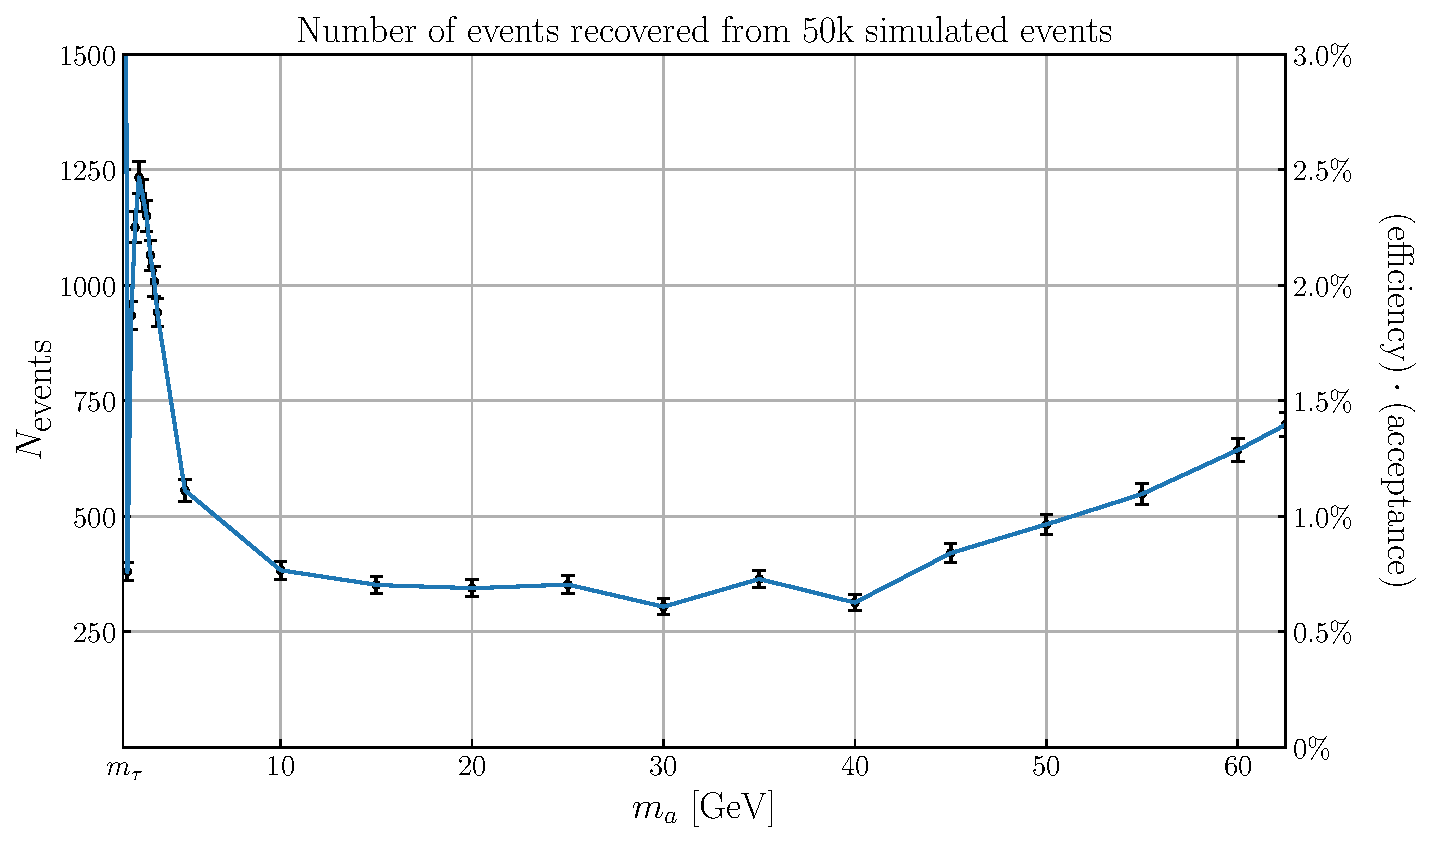
\includegraphics[width=0.8\linewidth]{figures/chapter5/H_to_OSSF0_efficiency.pdf}
    \caption[Monte-Carlo estimate of efficiency of CMS search for LFV Higgs-ALP decays.]{The number of OSSF0 events reconstructed from a simulation of $50\,000$ $h\rightarrow aa$ decay events in MadGraph for sample masses between $m_a = m_\tau$ and $m_a = m_h/2$. The signal efficiency is then estimated by taking the fraction of such events.}
    \label{fig:OSSF0_efficiency}
\end{figure}
In the study, the number of events with OSSF0 pairs predicted and observed at a luminosity of ${\cal L}=137~{\rm fb}^{-1}$ was 7. Following the analysis in Ref.~\cite{Feldman:1997qc}, the 95\% confidence interval on the Poisson mean for the number of signal events when the expected background and observed number of events are both $7$ is $(0, 6.81)$. A $95\%$ C.L. upper-limit on the branching fraction is then derived via
\begin{align}
    \epsilon \sigma_{\rm ggh}{\cal B}(h\rightarrow aa \rightarrow {\rm OSSF0}) \leq 6.81
\end{align}
where $\epsilon$ is the signal efficiency and acceptance. We can recast this constraint to a constraint on ${\overline C}_{ah}$ using the theoretical branching fraction for ${\cal B}(h\rightarrow aa \rightarrow {\rm OSSF0})$ and interpolating $\epsilon$ from Fig.~\ref{fig:OSSF0_efficiency} to all values of mass. The results of this constraint for ${\cal L} = 137~{\rm fb}^{-1}$ and a projected value of ${\cal L} = 3~{\rm ab}^{-1}$ are shown in the left panel of Fig.~\ref{fig:Cah_CMS}. For the projection, we take ${\cal L} = 3~{\rm ab}^{-1}$ assume that the number of observed and expected background events scale linearly with ${\cal L}$, which corresponds to a 95\% confidence interval on the Poisson mean of the number of signal events of $(0, 25.9)$. 

\begin{figure}[t!]
    \centering
    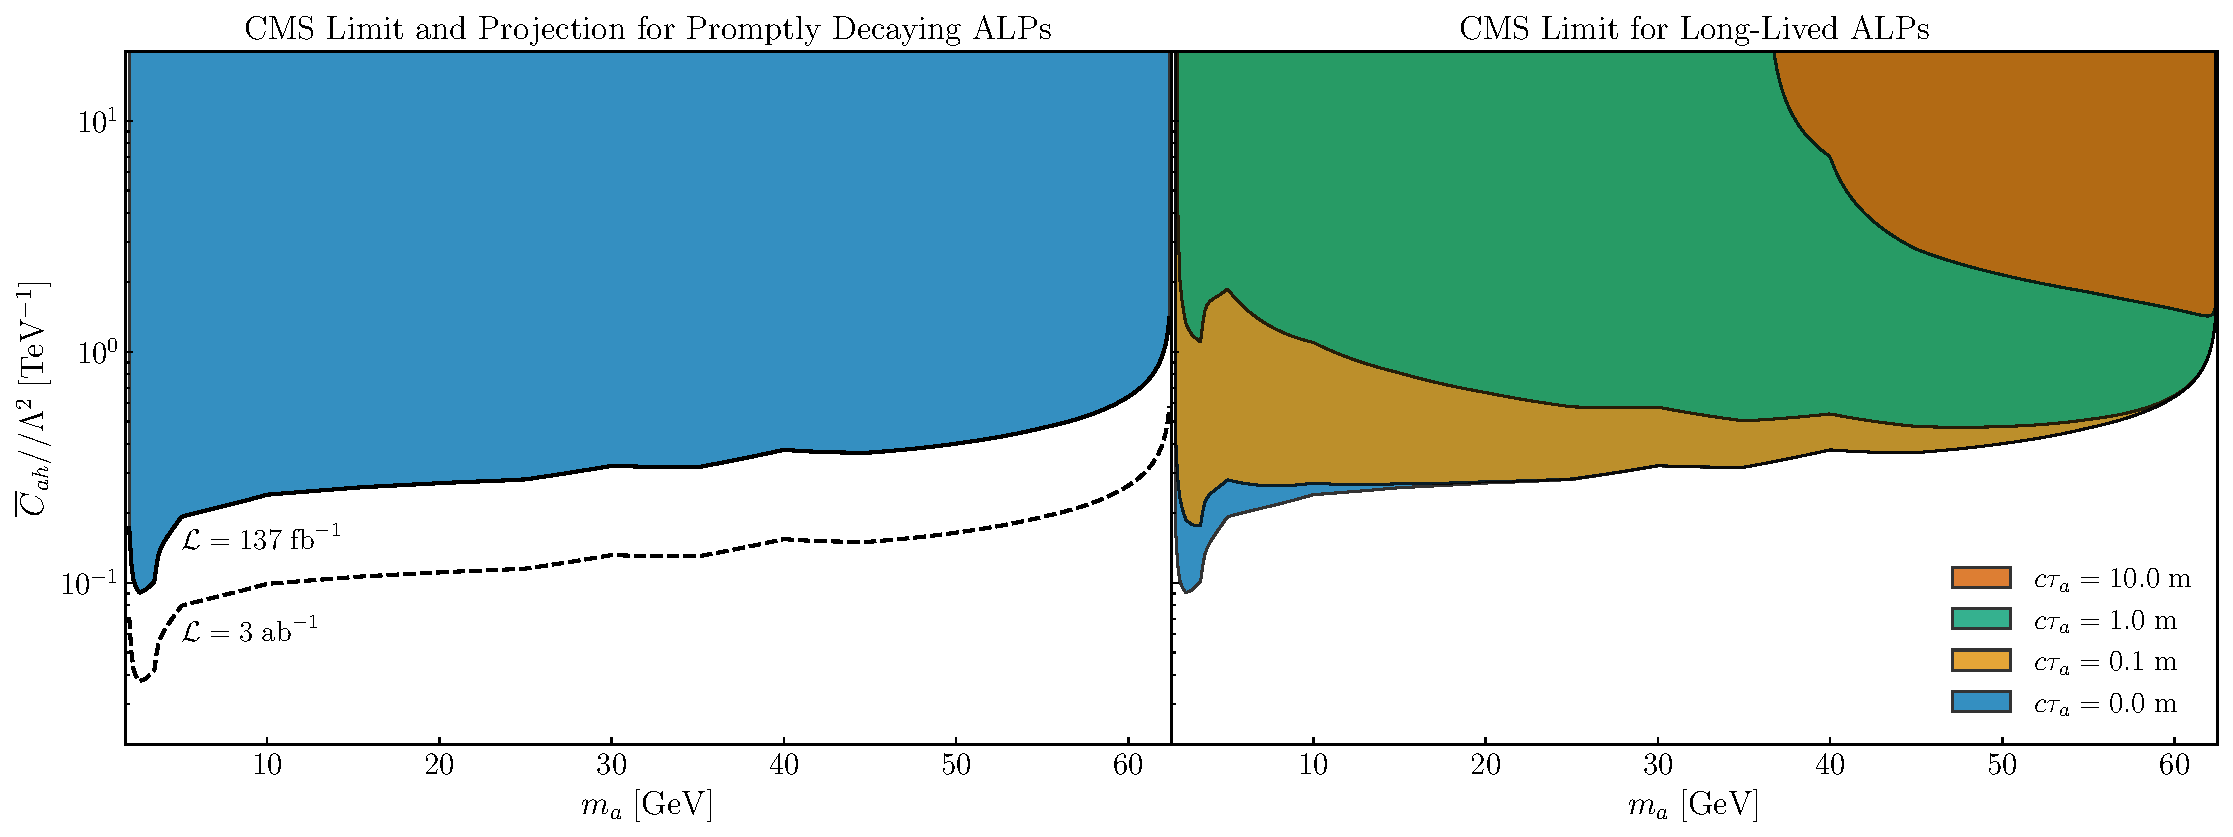
\includegraphics[trim={4cm 0 5cm 0}, width=\linewidth]{figures/chapter5/Cah_CMS_constraint.pdf}
    \caption[Limits on the effective Higgs-ALP coupling at CMS.]{(Left) Limits on the Higgs-ALP effective coupling $\overline{C}_{ah}$  according to the analysis performed in Ref~\cite{CMS:2019lwf}, assuming the ALP decays promptly. (Right) the same limits recast assuming the ALP has a non-zero lifetime $\tau_a$.}
    \label{fig:Cah_CMS}
\end{figure}

The analysis so far has operated under the assumption that the ALP decays promptly. However, some fraction of ALPs with long lifetimes will also decay within the CMS apparatus. The fraction of pair-produced long-lived ALPs which decay within a cylindrical detector of radius $L_{\rm det}$ is \cite{Bauer:2017ris}
\begin{align}
    f_{aa} = \int_0^{\pi/2}d\theta~\sin{\theta}\left(1-e^{-L_{\rm det}/(\gamma_a c \tau_a \sin{\theta})}\right)^2
\end{align}
where $\gamma_a$ is the boost of the ALP and $\tau_a = 1/\Gamma_a$ is the lifetime of the ALP in its rest frame. We take $\gamma_a \approx m_h/2m_a$, which is valid under the assumption that the Higgs is not heavily boosted. Taking ${L}_{\rm det} = 1.1~{\rm m}$ for the inner detector of CMS, we can recast the prompt constraints to account for long-lived ALPs by multiplying $f_{aa}$ to the signal efficiency $\epsilon$. These results are show in the right panel of Fig.~\ref{fig:Cah_CMS}. 


\subsection{Displaced ALP Decays at ATLAS and MATHUSLA}\label{sec:higgs_decay_ATLAS}
In addition to recasting prompt constraints to account for ALPs with long lifetimes, we can also examine constraints from searches for long-lived particles at CERN. One difficulty with such a task is that the main ditau decay mode of the ALP has a very high hadronic background (for example, from $B$ mesons) for displaced decays in the ATLAS or CMS inner detectors. As a result, we expect displaced decay analyses to become more important and fruitful when the ALP can travel into the muon spectrometer. This corresponds to $\tau_a\gtrsim1~{\rm m}$ or $C_{\tau \ell}/\Lambda \lesssim 10^{-5}~{\rm TeV}^{-1}$ for $m_a = 10~{\rm GeV}$. One work that considers such a scenario is Ref.~\cite{ATLAS:2022zhj}, which places constraints on the Higgs decaying into long-lived particles which have displaced jets in the final state by combining data from the ATLAS inner detector with data from the muon spectrometer. In particular, they consider the scenario in which one displaced jet is found in the inner detector and the other is found in the muon spectrometer. Since most of the ALPs in our model decay with at least one $\tau$ and most $\tau$s decay hadronically, this study can be used to constrain our model.

To adopt the work for our purposes, we digitize their results for a 95\% C.L. upper limit on the branching fraction for Higgs into two scalars using \verb|DigitizeIt| \cite{DigitizeIt}, then use a piecewise polynomial fit to generalize it to a variety of masses and lifetimes. The plots we digitize cover an extensive regions of lifetimes but are presented for only four masses: $m_a = 10$, $25$, $40$, and $55~{\rm GeV}$. Because of the limited data along the mass dimension, we account for the overfitting by interpolating plots for $m_a = 15$, $32.5$, and $47.5~{\rm GeV}$ using the geometric mean of the limits corresponding to the two nearest masses, then use these values along with the original masses to ensure that the fit function has a relatively smooth dependence along the mass dimension. The fit function agrees well with the data in regions of overlap, but we stress the results are likely to be accurate outside of the region $(10~{\rm GeV}, 55~{\rm GeV})$. For more accurate data in these mass regimes, the analysis of Ref.~\cite{ATLAS:2022zhj} would need to be repeated over a wide range of masses. the details of this fitting procedure can be found in the Github repository \cite{MarcarelliGithub2021}. While the details of this fit are unimportant for the exclusions presented in this section (which focus on the mass values studied in Ref.~\cite{ATLAS:2022zhj}), they are necessary to present exclusions in the $m_a$-$C_{\tau\ell}$ plane as is done in the next section.
\begin{figure}[t!]
    \centering
    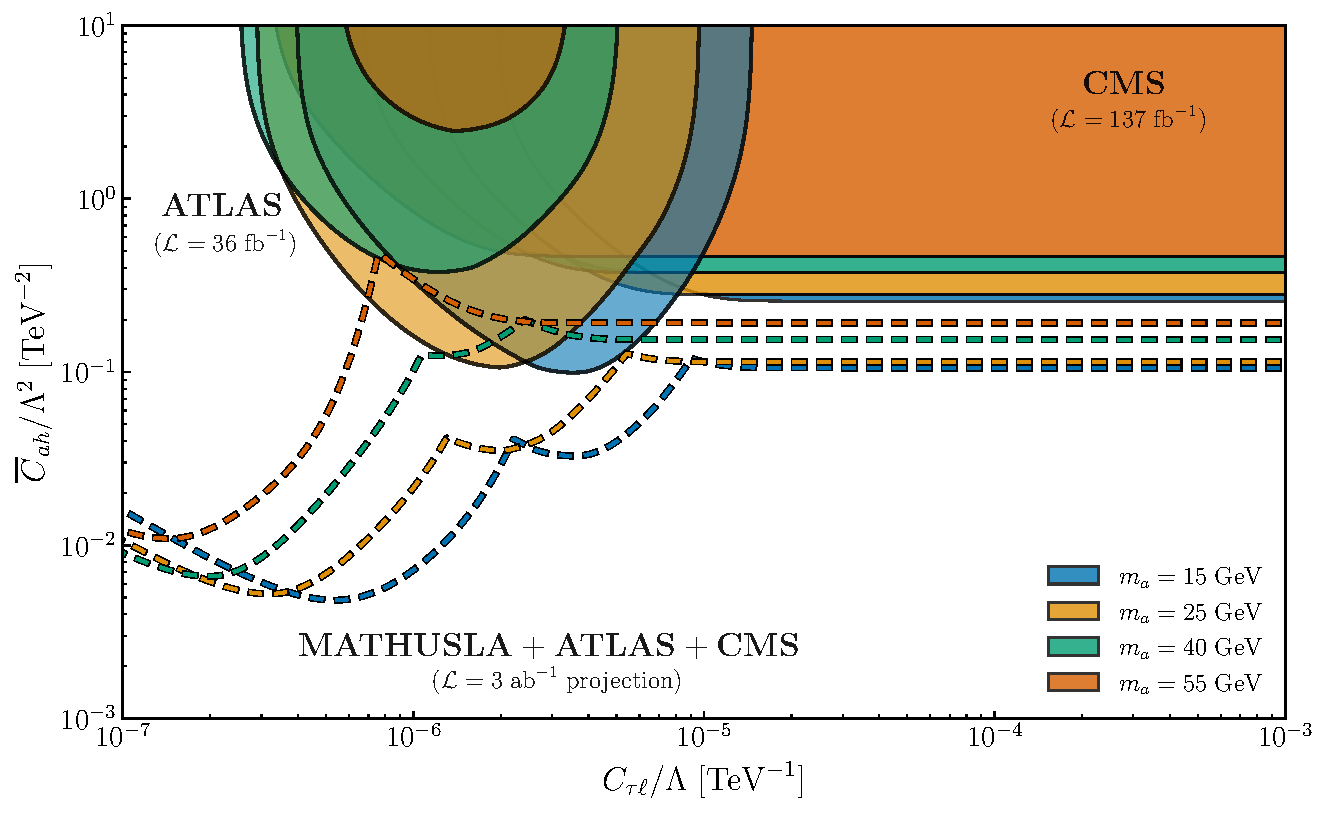
\includegraphics[width=\linewidth]{figures/chapter5/Cah_vs_Ctl_limits.pdf}
    \caption[Constraints on LFV ALP models at CMS, ATLAS, and MATHUSLA in the Higgs-ALP and lepton-ALP coupling plane.]{Exclusion plots for the Higgs coupling $C_{ah}$ and LFV coupling $C_{\tau \ell}$, for the masses $m_a = 10, 25, 40,$ and $55~{\rm GeV}$. The dashed lines encompass $3~{\rm ab}^{-1}$ projections from ATLAS and CMS, as well as the proposed MATHUSLA experiment.}
    \label{fig:Cah_Ctl_exclusion_all}
\end{figure}

It is also straightforward to generate projections for ${\cal L}=3~{\rm ab}^{-1}$ by assuming that the limits on the branching fraction scale inversely with $\sqrt{\cal L}$. However, stronger projections can be achieved by focusing on the community interest in dedicated long-lived particle detectors such as MATHUSLA \cite{Curtin:2018mvb,Lubatti:2019vkf,Alpigiani:2020tva,MATHUSLA:2025eth}, CODEX-b \cite{CODEX-b:2019jve}, ANUBIS \cite{Shah:2024fpl}, and SHiP \cite{SHiP:2021nfo}. Here we focus on the projected constraints for MATHUSLA in Ref.~\cite{Lubatti:2019vkf}, where the MATHUSLA detector is taken to be located on the surface of the Earth ($\sim100~{\rm m}$ above ATLAS and $100~{\rm m}$ down the beam pipe, with dimensions $100\times100\times20~{\rm m}^3$). An estimate is provided in Ref.~\cite{Curtin:2018mvb} for the projected constraint on the Higgs cross-section to long-lived particles:
\begin{align}
    (\epsilon \cdot \sigma)^{\rm MATH} &\approx \frac{4}{{\cal L} n_{\rm LLP} P^{\rm MATH}_{\rm decay}(c\tau)},\label{eq:MATH_LLP}\\
\intertext{with}
    P_{\rm decay}^{\rm MATH} &= \epsilon_{\rm geom}\left(e^{-L_2/\gamma c\tau} - e^{-L_1/\gamma c\tau}\right)
\end{align}
where $\gamma = m_h/2m_a$, $(L_1,L_2) = (200~{\rm m}, 230~{\rm m}),$ $\epsilon_{\rm geom} = 0.05$, and $n_{\rm LLP}$ is the number of long-lived particles in the Higgs decay channel. We find that this approximation works well for the projected exclusions of ${\cal B}(h\rightarrow aa)$ in Ref.~\cite{Curtin:2018mvb} at long lifetimes, provided that we take $(L_1, L_2) = (180~{\rm m},200~{\rm m})$ (due to the smaller detector size). At lower lifetimes, the approximation fails due to more complicated dependence on the detector acceptance and efficiency. Hence, for lower lifetimes, we fit the ${\cal B}(h\rightarrow aa)$ projected exclusions in Ref.~\cite{Curtin:2018mvb} with a polynomial fit, with the condition that it matches Eq.~\ref{eq:MATH_LLP} for $c\tau \gtrsim 10~{\rm m}$. Details of the fit can once again be found in the Github repository ~\cite{MarcarelliGithub2021}. The combined results of the ATLAS limits and projections, MATHUSLA projections, and CMS limits and projections are presented in Fig.~\ref{fig:Cah_Ctl_exclusion_all}. Rather than presenting exclusions in the $\overline{C}_{ah}$-$c\tau_a$ plane, we present exclusions in the $\overline{C}_{ah}$-$C_{\tau \ell}$ plane under the assumption of universal couplings, i.e. $C_{\tau e} = C_{\tau \mu} = C_{\tau\tau}$. As long as the Higgs-ALP coupling is substantial, we see that both the ATLAS and CMS constraints can probe the LFV couplings far beyond the limits from LFV leptonic decays in Fig.~\ref{fig:LFV_limits}. 

\subsection{Combined Limits on LFV Couplings}\label{sec:higgs_combined}
Here we present the combined results from LFV leptonic decays, prompt decays, and displaced decays. To do so, we present exclusion plots on the off-diagonal coupling $C_{\tau \ell}$ in the event that all couplings (or at the very least, those couplings to the $\tau$) are universal. We note that limits on $C_{\tau \ell}$ as a function of the ALP mass are dependent on the size and nature of the ALP-Higgs coupling. The terms $C_{ah}$ and $C_{ah}'$ are both present for, e.g., the pion in the SM: $C_{ah}$ arises through a Higgs-gluon effective coupling due to heavy quark loops, whereas $C_{ah}'$ arises from Yukawa couplings with the lighter quarks. Hence, which of the Higgs couplings is present likely depends on the UV nature of the LFV ALP. Since the $C_{ah}'$ coupling is multiplied by a factor of $m_a^2/m_h^2$ in the interaction term (\ref{eq:ALP_Higgs_int}), the most relevant Higgs coupling is $C_{ah}$ for light ALP masses. However, in scenarios with a heavy composite ALP in a theory with only light quarks which couple to the Higgs, such as the model in Ref.~\cite{Davoudiasl:2017zws}, $C_{ah}'$ is the only significant ALP-Higgs coupling. All limits and projections are presented at the 95\% C.L.. The limits are demonstrated in Fig.~\ref{fig:LFV_ALP_limits}.

\begin{figure}[t!]
    \centering
    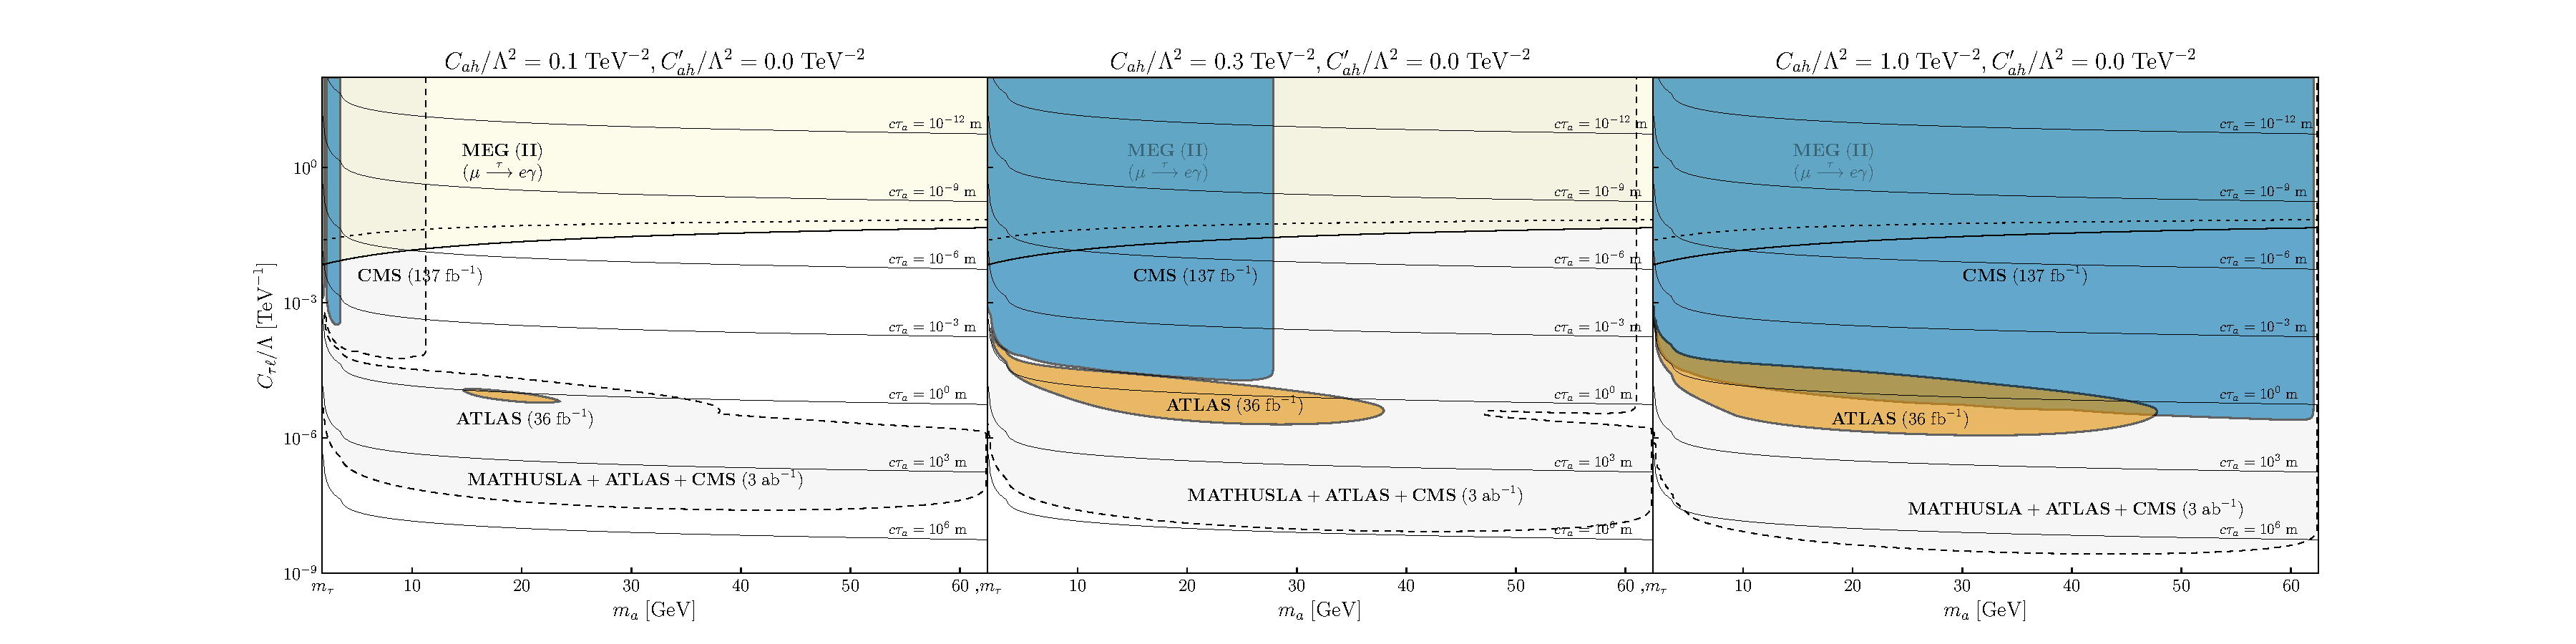
\includegraphics[trim={8cm 0 8cm 0}, width=\linewidth]{figures/chapter5/Ctl_vs_ma_limits_Cahp=0.pdf}
    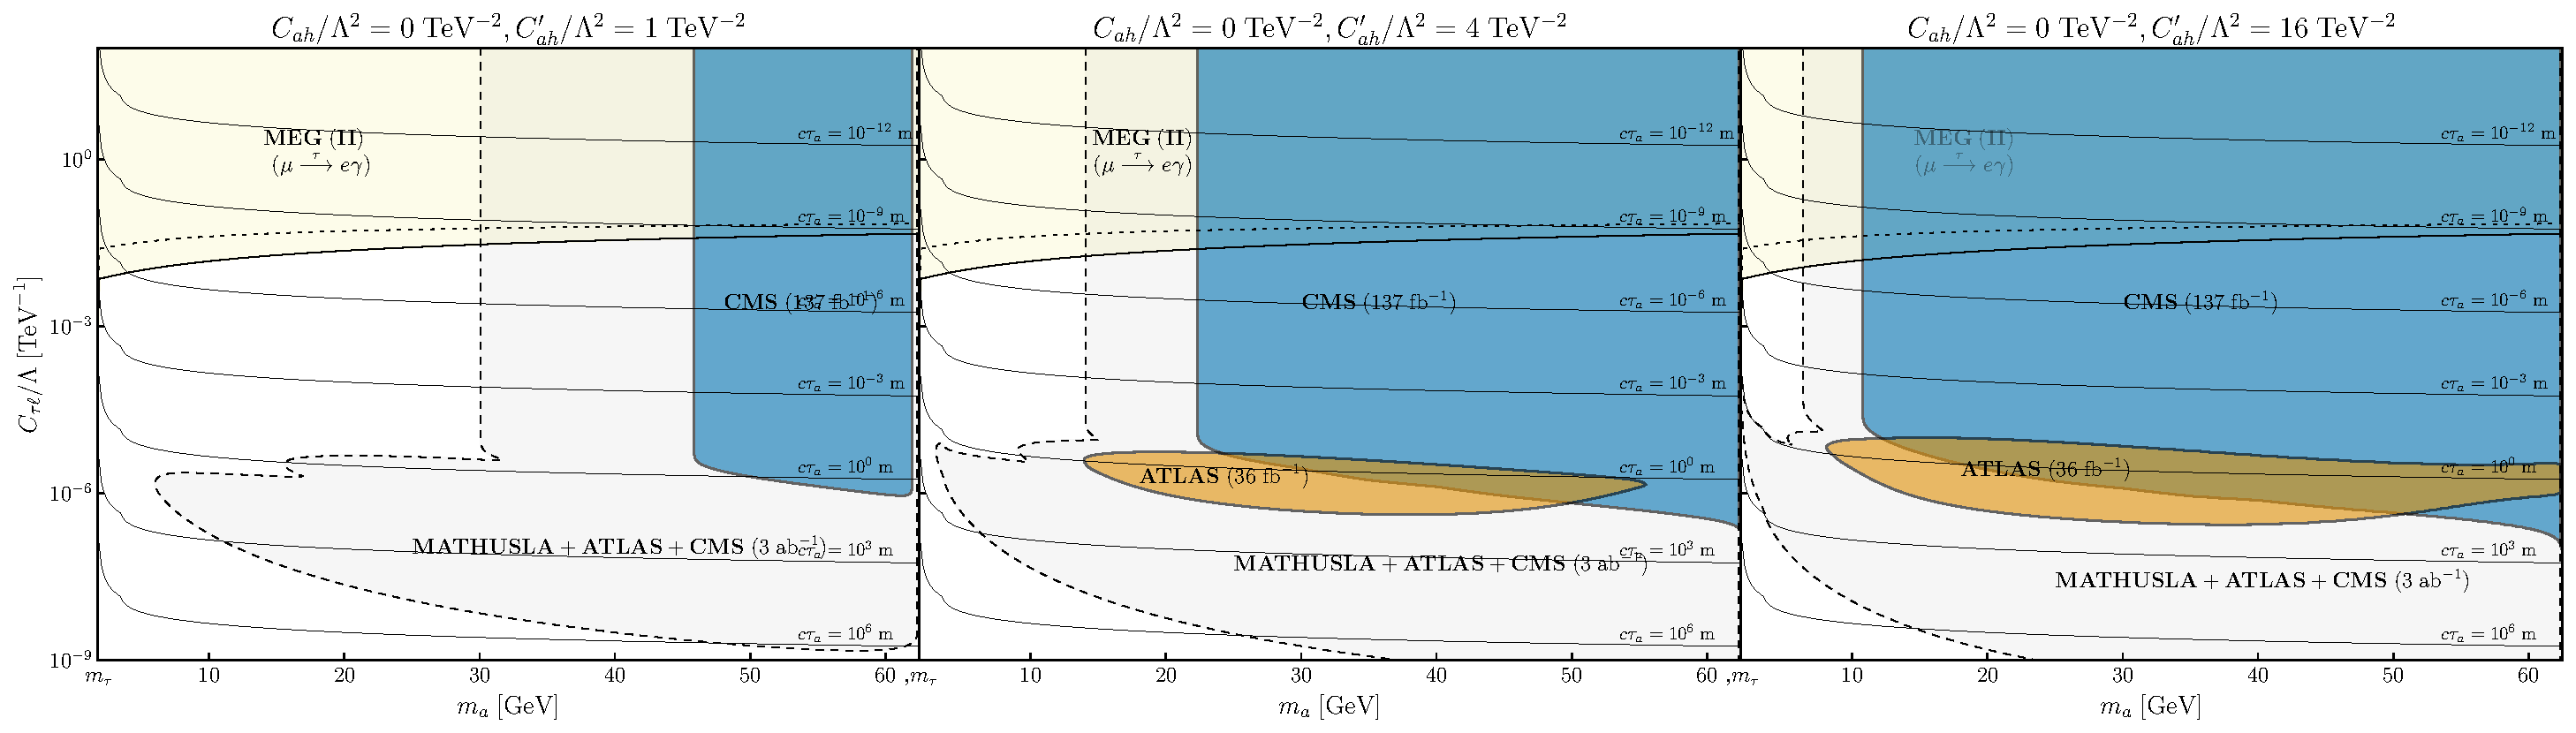
\includegraphics[trim={8cm 0 8cm 0}, width=\linewidth]{figures/chapter5/Ctl_vs_ma_limits_Cah=0.pdf}
    \caption[Constraints on LFV ALP models at CMS, ATLAS, and MATHUSLA in the ALP mass and lepton-ALP coupling plane.]{Combined limits on the leptophilic LFV ALP model considered in this section, over a range of different Higgs interaction couplings. Limits from LFV lepton decays are presented in yellow, with the leading limit coming from $\mu \rightarrow e\gamma$ through an internal $\tau$. Limits from Higgs decays at CMS are shown in blue, and at ATLAS are shown in orange. Finally, combined projections from CMS, ATLAS, and MATHUSLA assuming ${\cal L} = 3~{\rm ab}^{-1}$ of integrated luminosity are shown in gray.}
    \label{fig:LFV_ALP_limits}
\end{figure}

 While one may expect that the leading limits on $C_{\tau \ell}$ from LFV lepton decays to come from the branching limit on ${\cal B}(\tau\rightarrow \ell\gamma)$, this is only true if the off-diagonal couplings are small compared to the diagonal couplings. In the universal scenario we are considering, the leading constraint comes from $\mu \rightarrow e\gamma$ due to the mass-enhancement of the diagram with an internal $\tau$. In particular, the leading limit on the branching fraction ${\cal B}(\mu \rightarrow e\gamma)$ comes from the MEG experiment with ${\cal B}(\mu \rightarrow e\gamma) < 4.2\times10^{-13}$, and this can be directly converted into a limit on $\sqrt{C_{\tau\mu}C_{\tau e}}/\Lambda$, as is done in the bottom left panel of Fig.~\ref{fig:LFV_limits}. We reproduce these limits in yellow in Fig.~\ref{fig:LFV_ALP_limits}. The solid and dashed lines correspond to PC and chiral ALPs, respectively.

For significant Higgs-portal interactions, we see that the LHC provides competitive constraints for the $C_{\tau \ell}$ coupling of the ALP. However, regardless of the value of the Higgs portal coupling, the model is relatively unconstrained for $C_{\tau\ell}/\Lambda \lesssim 10^{-6}~{\rm TeV}^{-1}$ due to the lifetime of the produced ALPs. Hence, there is a lot of unexplored potential for the long-lived ALPs which could potentially be discovered or ruled out by proposed detectors like MATHUSLA. 

Finally, we note that for low enough Higgs coupling, the only significant constraints on the ALP-lepton coupling come from the LFV lepton decays. In this case, the limits presented are on a product of two couplings, so certain models with exotic hierarchies between the couplings (in the extreme case, only $C_{\tau \ell} \neq 0$) will completely evade these constraints as well. We will explore this scenario in the next few sections in the context of ALP production from lepton-nucleus collisions, where a singular ALP coupling can be isolated and constrained, hence providing an absolute limit on the coupling. 

While we have focused on LFV ALPs, our results apply with limited modification to flavor-conserving leptophilic ALPs as well. In particular, each of the analyses we have conducted still have non-zero signals for the decay $h\rightarrow aa \rightarrow \tau^\pm \tau^\mp$. For the ATLAS analysis, all that matters is the identification of pairs of displaced jets, which is indeed more likely in the $h\rightarrow aa\rightarrow \tau^\pm\tau^\mp$ scenario, and for the MATHUSLA scenario, the final-states of the long-lived particle are unimportant as long as they're identifiable. Hence, the only limit which is noticeably weakened is the prompt CMS limit, because it relies on each $\tau$ decaying leptonically. This has the effect of multiplying the limits in Fig.~\ref{fig:LFV_ALP_limits} by a factor of $3$. The ALP-Higgs and diagonal ALP-$\tau$ coupling are probed in Fig.~30 of Ref.~\cite{Bauer:2017ris}; we note that while their results rely on a different analysis than ours, the limits we achieve are comparable in magnitude.


\section{LFV ALP Production at The EIC}\label{sec:EIC_ALP}

The EIC is expected to greatly improve our understanding of the strong interactions within heavy nuclei once it begins operation in the 2030s. We have previously considered an alternate possibility for the electron-nucleus collisions at the EIC in Chapter \ref{upc}: namely, production of GeV-scale particles at the EIC through coherent electron-ion collisions, in which the electromagnetic interaction between the electron and the nucleus is enhanced by the number of protons in the nucleus. Here, we consider the possibility of probing the LFV coupling between an ALP and the flavor-changing $e$-$\tau$ current, $C_{\tau e}/\Lambda$, directly at the EIC via coherent production of the ALP, according to the process $e^- A_Z \rightarrow \tau^- A_Z a$. We will assume that the EIC is in gold mode, with $E_e = 18~{\rm GeV}$ and $E_{\rm Au} = 110~{\rm GeV}/{\rm nuc}$. In the last section, we considered ``democratic'' coupling of the ALPs to the leptons. Here, we consider the opposite extreme: an ALP with a singular $C_{\tau e}$ coupling. The EIC is uniquely poised to probe this region of the parameter space, and it also coincides with LFV ALP explanations to the electron $g-2$ anomalies that are not yet ruled out by other experiments.

Given that we are focused on a single coupling, we have the relatively simple interaction Lagrangian
\begin{align}
    {\cal L}_{\rm int.} &= -\frac{\partial_\mu a}{\Lambda} C_{\tau e}\bar{\tau}\gamma^\mu( \sin{\Theta} + \cos{\Theta}\gamma^5)e + {\rm H.c.}
\end{align}
We ignore CP-violating phases in this discussion, as any non-zero phase will likely be ruled out by the electron EDM constraints in Fig.~\ref{fig:EDM_limits}. However, we do allow a PV angle $\Theta$ in the interaction. The EIC cross-section is only dependent on this PV angle at ${\cal O}(m_e/m_\tau)$, so the limits obtained on $C_{\tau e}$ from this section are essentially independent of the PV nature of the interaction. We are agnostic to the UV origins of such an interaction, but we point out that it is perturbatively protected by a ${\Bbb Z}_4$ symmetry with $Q(e) = i$, $Q(\tau)  = -i$, and $Q(a) = -1$. Hence, one can expect that such a term will survive higher-order corrections from renormalization.


\subsection{Detector Capabilities}\label{sec:EIC_ALP_detector}

For the expected capabilities of the EIC detector apparatus, we refer to the {\it Detector Requirements} section of the EIC Yellow Report \cite{AbdulKhalek:2021gbh}. For our purposes, we will assume that the EIC is operating in gold mode, with $E_e = 18~{\rm GeV}$ and $E_{\rm Au} = 110~{\rm GeV}/{\rm nuc}$. In the rest frame of the nucleus, this corresponds to an electron energy of $E = 4.2~{\rm TeV}$, so this collision can be likened to a $4.2~{\rm TeV}$ beam dump. It is reasonable to expect that a collision of this energy can produce GeV-scale ALPs. We take an integrated luminosity of ${\cal L} = (100/A)~{\rm fb}^{-1}$, corresponding to about one year of operation in ion mode (assuming $L = 10^{34}~{\rm cm}^2/{\rm sec}$ luminosity).

Of course, it is not enough to produce such particles, we must also be able to detect them. From the discussion in  Section \ref{sec:phi_kin}, we can expect that many of the ALPs which are produced have a high pseudorapidity. The Yellow Report indicates the EIC will have full coverage of $|\eta| < 3.5$ \cite{AbdulKhalek:2021gbh}, although the B0 spectrometer on the ion-side of the interaction is expected to have a coverage up to $|\eta| < 6$ \cite{Adkins:2022jfp}. Given that the ALPs are produced off of the lepton-side of the interaction, they mostly end up on the electron-side of the detector, so we take $|\eta| < 3.5$ for our study. Examining Fig.~\ref{fig:pseudorapidity_IQR}, we see that for scalars produced via $e$-$\tau$ conversion, $|\eta| < 3.5$ is sufficient to capture a majority of GeV-scale particles produced in this way at the EIC. 

\subsection{Signal and Background} \label{sec:EIC_ALP_BG}

Given the simplicity of the model, the only possible production mode is $e^- A_Z \rightarrow \tau^- A_z a$.\footnote{Even in the event that other leptonic couplings are present, this is by far the most dominant production mode, since the ALP coupling is proportional to the mass of the leptons in the vertex.} There are then two possible decay modes for the ALP: $a \rightarrow e^- \tau^+$ and $a\rightarrow e^+\tau^-$. The former is lepton-flavor conserving, so it will be overwhelmed with SM background. Hence, we focus on the decay mode $a \rightarrow e^+ \tau^-$. We will leverage the LFV nature of the final state by vetoing on identification of an electron $e^-$, and requiring identification of the $e^+$ and one of the $\tau^-$. 

\begin{figure}[t!]
    \centering
    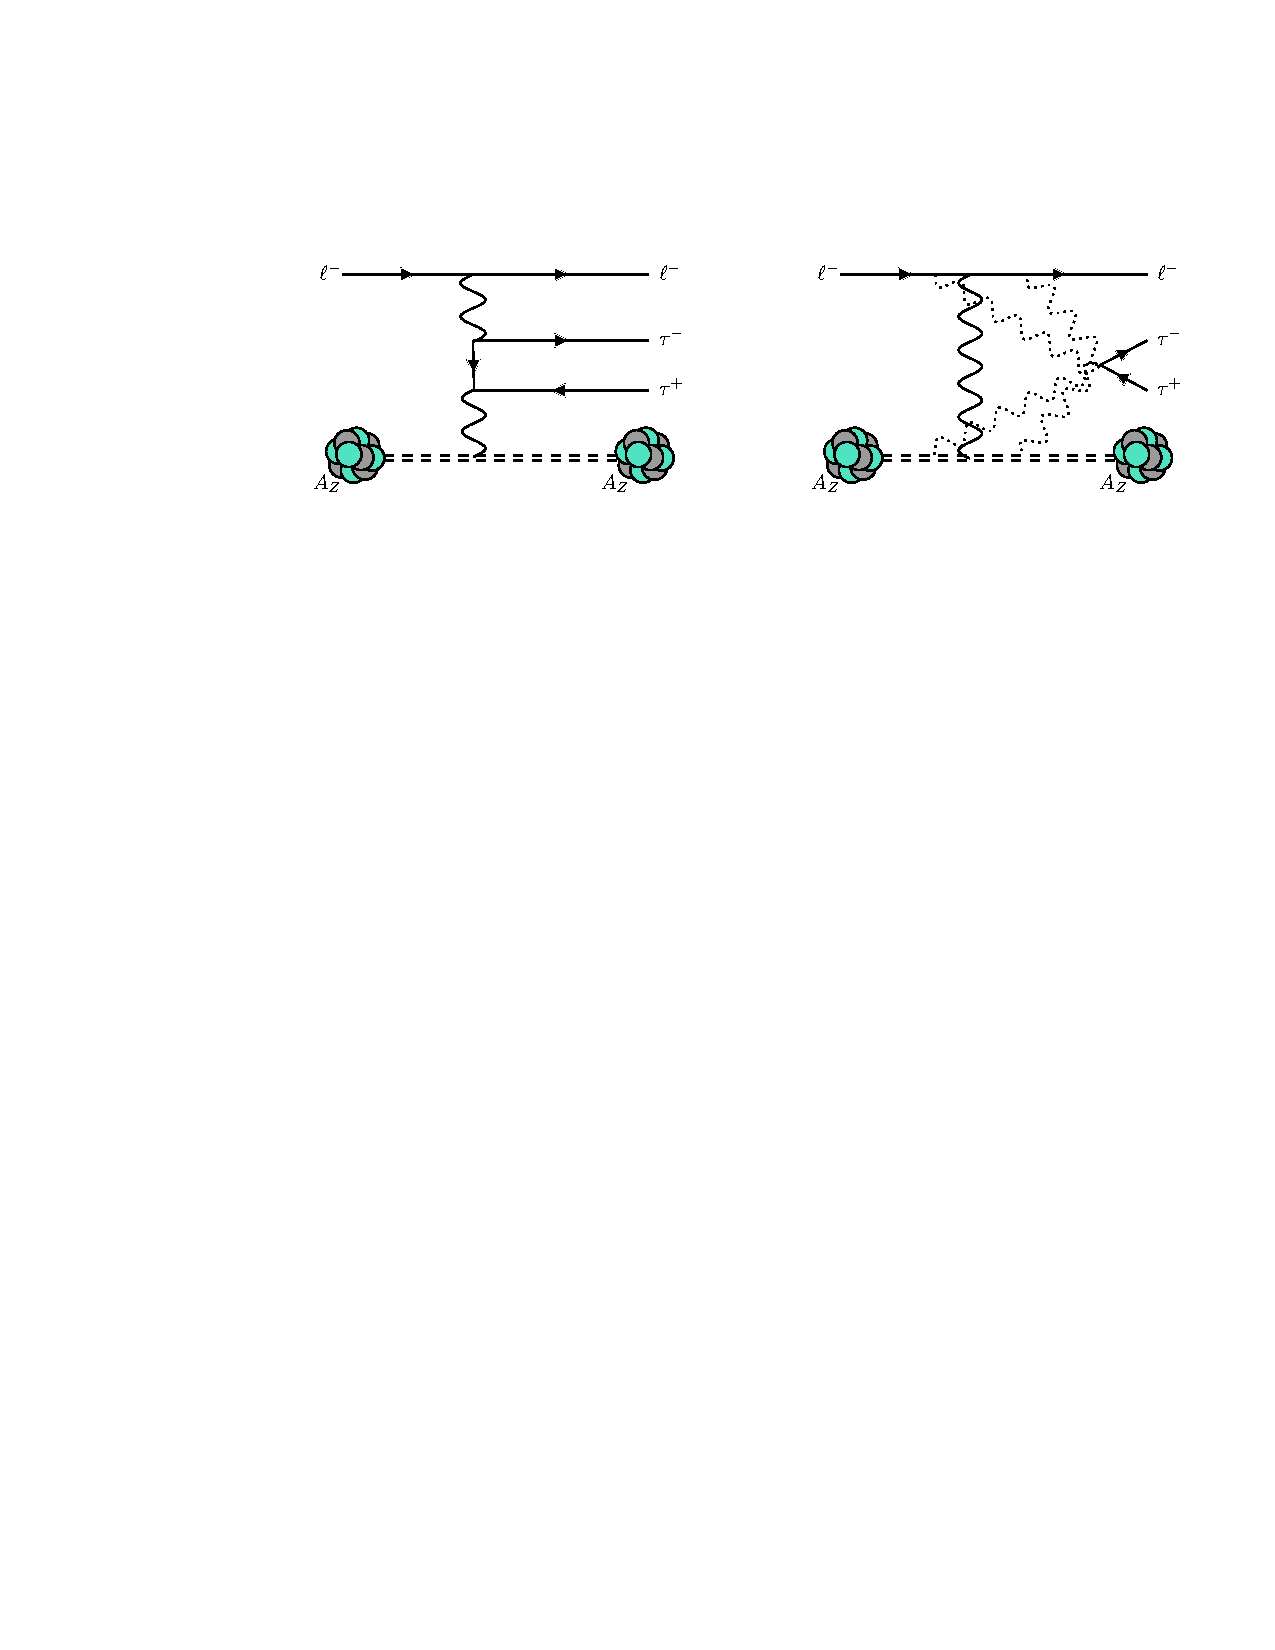
\includegraphics[width=\linewidth]{figures/chapter5/ditau.pdf}
    \caption[Ditau production process at lepton-ion collider experiments.]{Diagrams for ditau production which contribute to the background for the collision $\ell^- A_Z \rightarrow \tau^- A_Z (a \rightarrow \ell^+\tau^-)$ at the EIC and MuSIC, particularly when the $\ell^-$ is lost down the beam-pipe and the $\tau^+$ decays to $\ell^+\bar{\nu}\nu$. The dashed photon lines in the diagram on the right indicate that the $\tau$ pair production can occur from a photon off of any one of the legs. }
    \label{fig:ditau_background}
\end{figure}

The largest source of background is ditau production $e^- A_Z \rightarrow e^- A_Z \tau^+\tau^-$, through one of the diagrams shown in Fig.~\ref{fig:ditau_background}. This can mimic $e^- A_Z \rightarrow \tau^- A_z (a\rightarrow e^+ \tau^-)$ if the $\tau^+$ decays leptonically and the final-state electron is lost down the beam pipe. A rough estimate of the cross-section for ditau production at the EIC can be gleaned from Ref.~\cite{Bulmahn:2008fa}, which computes the cross-section for ditau production from cosmic-ray muons incident on rock (which is assumed to be $_{\scriptsize 11}^{\scriptsize 22}{\rm Na}$). Focusing on the energy $E \approx 4~{\rm TeV}$ (the energy of the electron at the EIC in the frame of the nucleus) in  Fig.~3 of the reference and assuming the cross-section is enhanced by $(Z_{\rm Au}/Z_{\rm Na})^2 \approx 50$ at the EIC, we estimate $\sigma_{\rm b.g.} \approx 2.6\times10^{4}~{\rm pb}$. This cross-section is quite large, but as suggested previously, the majority of it can be mitigated by vetoing on the identification of an $e^-$. Even so, there is a possibility that the incident electron in the SM ditau production process is either lost down the EIC beam-pipe or mis-identified as an $e^+$. We take $10^{-2}$ for the rate of electron loss, in line with the proposed detector requirements for the EIC \cite{AbdulKhalek:2021gbh}. We assume the rate of electron misidentification as a positron is $10^{-3}$, similar to the rate of a pion faking an electron from simulations in Ref.~\cite{AbdulKhalek:2021gbh}. Finally, for the $\tau$ identification rate, we consider two scenarios: $\epsilon_\tau = 1\%$ in line with the analysis done in Ref.~\cite{Zhang:2022zuz}, and the more optimistic scenario $\epsilon_\tau \approx 10\%$, which corresponds to reconstruction of all three-prong $\tau$ decays. 


\subsection{Combined Limits}\label{sec:EIC_ALP_limits}

Using the analysis above, the background efficiency is $\epsilon_{\rm b.g.} \approx 0.0036\epsilon_\tau$, and the signal efficiency is $\epsilon_{\rm sig.} = \epsilon_\tau/2$, where the factor of $1/2$ takes into account the fact that the final-state ALP must decay to $e^+\tau^-$. For ${\cal L} = 100/A~{\rm fb}^{-1}$, this corresponds to $N_{\rm b.g.} = 47000\epsilon_\tau$ background events. To place $95\%$ C.L. ($2\sigma$) limits on the coupling $C_{\tau e}/\Lambda$, we find the value of $C_{\tau e}/\Lambda$ for which the number of expected signal events is $N_{\rm sig} = 2\sqrt{N_{\rm b.g.}} \approx 430\sqrt{\epsilon_\tau}$. Letting $\hat{\sigma}$ represent the cross-section normalized by $(C_{\tau e}/\Lambda)^2$, we have
\begin{align}
    \frac{C_{\tau e}}{\Lambda} \leq \sqrt{\frac{430}{\sqrt{\epsilon_\tau}\hat{\sigma} {\cal L}}}~{\rm TeV}^{-1}.
\end{align}
\begin{figure}[t!]
    \centering
    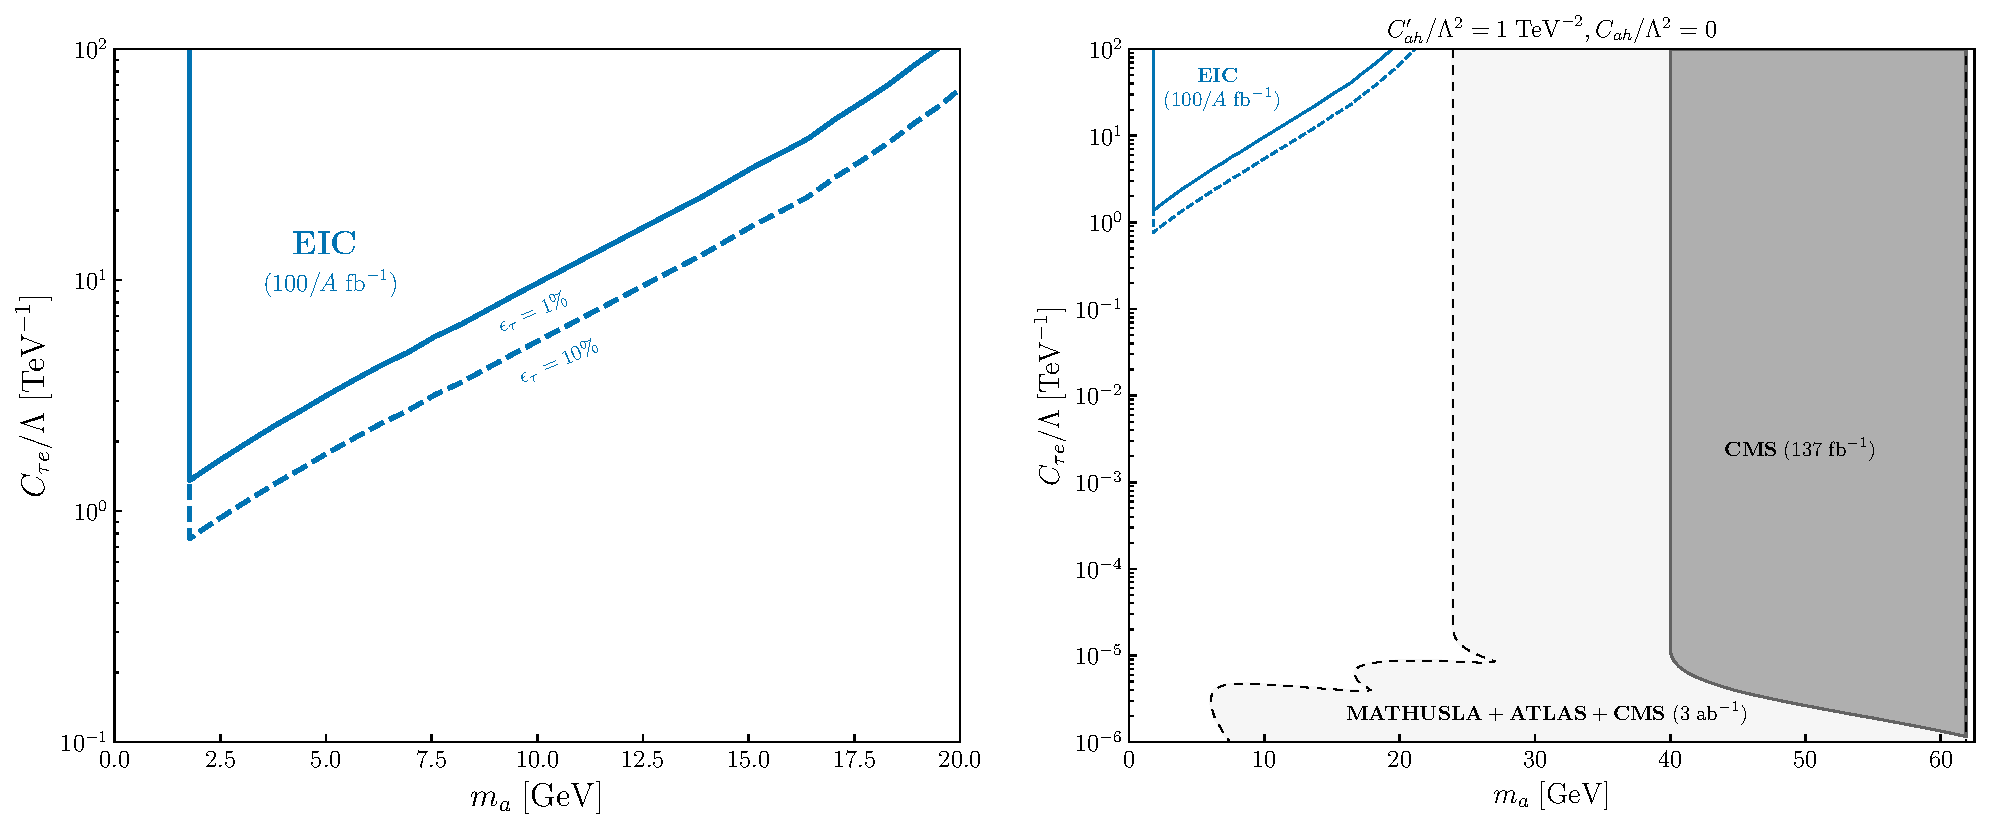
\includegraphics[width=\linewidth]{figures/chapter5/EIC_ALP_limits.pdf}
    \caption[Projected constraints on LFV ALPs at the EIC.]{(Left) limits on the LFV coupling $C_{\tau e}/\Lambda$ from the EIC assuming a $\tau$ efficiency of $\epsilon_\tau = 1\%$ (blue, solid) and $\epsilon_\tau = 10\%$ (blue, dashed). (Right) the same limits in the larger context of the LHC Higgs decay limits from the last section, assuming $C_{ah}'/\Lambda^2 = 1~{\rm TeV}^{-2}$ and $C_{ah}/\Lambda^2 = 0~{\rm TeV}^{-2}$. These limits are recast for the scenario in which $C_{\tau e}$ is the only non-zero coupling of the ALP.}
    \label{fig:EIC_ALP_limits}
\end{figure}

The resulting bounds on $C_{\tau e}/\Lambda$ are shown in the left panel of Fig.~\ref{fig:EIC_ALP_limits}, with $\epsilon_\tau = 1\%$ represented as a solid blue line and $\epsilon_\tau = 10\%$ represented as a dashed blue line. The right panel shows the same limits as in the left panel, but in the context of the LHC Higgs decay limits and projections from the previous section with a representative value of the Higgs-ALP coupling of $C_{ah}'/\Lambda^2 = 1~{\rm TeV}^{-2}$ and $C_{ah}/\Lambda^2 = 0~{\rm TeV}^{-2}$. These limits have been recast for the scenario where $C_{\tau e}$ is the only non-zero coupling. While the reach at the LHC is much stronger than the reach at the EIC, it is dependent on both the strength and nature (i.e. whether $C_{ah}$, $C_{ah}'$, or both are present) of the Higgs-ALP interaction. Hence, there are still scenarios (such as that shown in the second panel of Fig.~\ref{fig:EIC_ALP_limits}) for which the EIC is in a unique position to probe the theory.

Although we have focused on the scenario where the ALP only couples to $e$ and $\tau$, our results are mostly insensitive to this choice. In the presence of other LFV couplings, our results are essentially constraints on $\sqrt{{\cal B}(a\rightarrow e\tau)}C_{\tau e}/\Lambda$, with the caveat that the $a\rightarrow \tau^+\tau^-$ decay mode could also contribute to the signal if $\tau^+ \rightarrow e^+\bar{\nu}\nu$. In this more general scenario, the reach of the EIC is mostly ruled out by the limits from LFV leptonic decays $\tau \rightarrow 3\ell$ and $\tau \rightarrow \ell \gamma$, shown at the bottom of Fig.~\ref{fig:LFV_limits}. Hence, while the limits placed from the EIC on $C_{\tau e}$ are weaker, they can be seen as {\it absolute} limits on the coupling, as any larger value of $C_{\tau e}$ would be completely ruled out at the EIC, almost entirely irrespective of the other ALP couplings. 

Finally, we note that the ditau background can be entirely avoided by requiring positive identification of {\it both} $\tau$s in the final state, along with the $e^+$. We have avoided this possibility given the experimental difficulty involved in resolving multiple $\tau$s, but if methods improve on this front then this approach may be preferable. One may also be able to leverage other LFV final-states of the ALP decay (e.g., those involving muons) for additional background-free signal events; however, even a complete reduction of background for such processes will not be enough for the EIC to compete with the stringent constraints on $\sqrt{C_{\mu \tau}C_{e\tau}}/\Lambda$ from  the MEG limit on the $\mu\rightarrow e\gamma$ branching fraction.


\begin{figure}[t!]
    \centering
    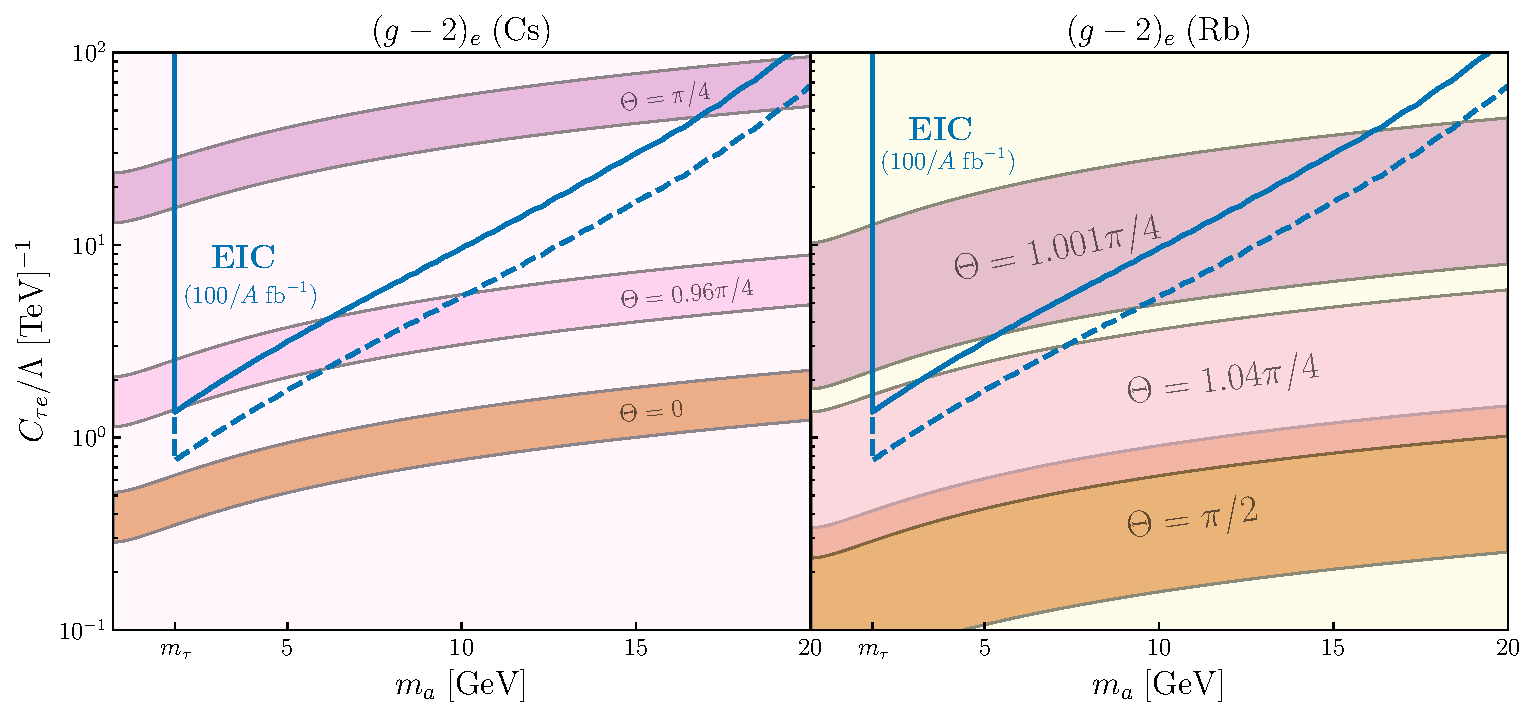
\includegraphics[width=\linewidth]{figures/chapter5/EIC_ALP_electron_g_2.pdf}
    \caption[Projected constraints on LFV ALPs at the EIC, alongside explanations for the electron $g-2$ anomalies.]{Expected limits on $C_{\tau e}/\Lambda$ from the EIC, alongside explanations for the electron $g-2$ anomalies for different PV angles $\Theta$. The left panel presents $2\sigma$ explanations for the anomaly obtained from using $\alpha({\rm Cs})$, and the right panel presents explanations for the anomaly obtained from using $\alpha({\rm Rb})$.}
    \label{fig:EIC_g_2}
\end{figure}

\begin{figure}[t!]
    \centering
    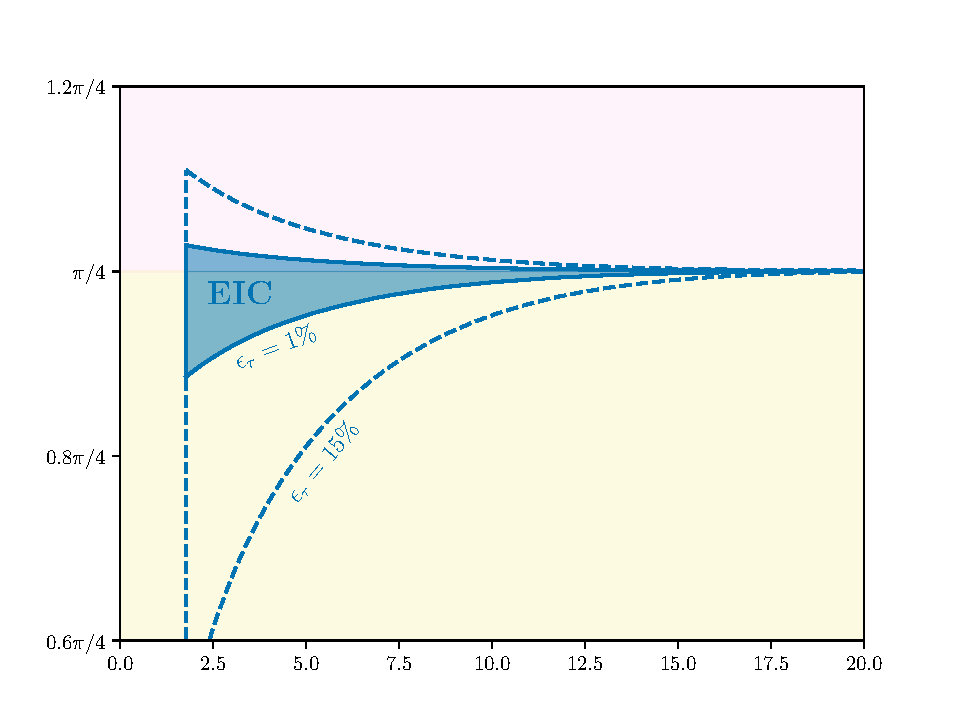
\includegraphics[width=0.6\linewidth]{figures/chapter5/EIC_g_2_probe.pdf}
    \caption[Region in the $m_a$-$\Theta$ plane for which the EIC probes an LFV ALP explanation to either of the electron $g-2$ anomalies.]{The region in the $m_a$-$\Theta$ plane for which the EIC probes an LFV ALP explanation to either of the electron $g-2$ anomalies.}
    \label{fig:EIC_g_2_region}
\end{figure}

\subsection{Explanations to $(g-2)_e$}\label{sec:EIC_ALP_g_2}

The reach of the EIC turns out to coincide with the $C_{\tau e}$ required to explain either of the electron $g-2$ anomalies, per the discussion in Section \ref{sec:g-2_explanation}. In particular, the sign of the contribution to $a_e$ is dependent on the PV angle, so PV angles $\Theta < \pi/4$ are able to explain the anomaly obtained from using $\alpha({\rm Cs})$, whereas PV angles $\Theta > \pi/4$ are able to explain the anomaly obtained from using $\alpha({\rm Rb})$. To illustrate this point, we plot the EIC constraints alongside $2\sigma$ explanations to each anomaly in Fig.~\ref{fig:EIC_g_2}, for three representative angles. We find that the EIC is equipped to probe near-chiral explanations of the electron $g-2$ anomalies, which can occur if the ALP's coupling to right-handed leptons is suppressed relative to its coupling to left-handed leptons, or vice-versa. If one takes the more optimistic $\tau$ efficiency $\epsilon_\tau = 10\%$, the EIC is {\it just} able to probe the upper end of the $2\sigma$ band for $\Delta a_e{(\rm Cs)}$ with $\Theta = 0$ (and hence will also have non-zero overlap with the $2\sigma$ bands for all $\Theta > 0$).


To get a better sense of which anomaly explanations the EIC is sensitive to, we can compute the region in the $m_a$-$\Theta$ plane for which the EIC limit intersects the center of the bands shown in Fig.~\ref{fig:EIC_g_2}. The resulting region is presented in Fig.~\ref{fig:EIC_g_2_region}, with the conservative ($\epsilon_\tau = 1\%$) scenario shaded in blue and the optimistic ($\epsilon_\tau = 10\%$) scenario a dashed blue line. This reinforces the point that the EIC is mostly able to probe near-chiral solutions to the electron $g-2$ anomalies, although the angle can deviate farther from $\pi/4$ for lower masses.


\section{LFV ALP Production at MuBeD and MuSIC}\label{sec:MuBeD_MuSIC_ALP}
With interest growing in the particle physics community for a multi-TeV muon collider \cite{Delahaye:2013jla,Long:2020wfp,Accettura:2023ked}, it is likely that intermediate experiments involving TeV muon beams are in our future. We have discussed two possibilities for such experiments in Chapter \ref{upc}, namely a TeV muon beam dump (MuBeD) and a Muon (Synchrotron) Ion Collider (MuSIC). In this section, we will examine the degree to which such experiments would be able to probe the LFV ALP model. We will once again focus on coherent production of an ALP $a$ via the process $\mu^- A_Z \rightarrow \tau^- A_Z a$, which will allow us to probe the $C_{\mu \tau}$ coupling. Similar to the previous section, we will assume that this is the only non-zero coupling of the ALP to the leptons, so that the interaction term is
\begin{align}
    {\cal L}_{\rm int} = C_{\tau\mu}\frac{\partial_\mu a}{\Lambda}\bar{\tau}(\sin{\Theta}+\cos{\Theta}\gamma^5)\mu + {\rm H.c.}
\end{align}

\subsection{Detector Capabilities}\label{sec:MuSIC_MuBeD_ALP_detector}
We are years of research and development away from a functioning TeV muon beam. As such, no serious prototype has yet been put forward for either MuBeD or MuSIC, so here we will speculate about reasonable detector requirements and geometry one might expect for these experiments. 

\begin{center}
{\it 1. Muon Beam Dump (MuBeD)}
\end{center}

Here, we consider the possibility of a 1 TeV muon fixed target experiment, similar to the experiments investigated in Refs.~ \cite{Cesarotti:2022ttv,Cesarotti:2023sje}. Such an experiment could be constructed as one component of the muon collider facility, or developed even earlier during the muon beam research and development phase. The original proposal considers a TeV-energy muon beam dumped on a thick target ($\sim 10~{\rm m}$) along with a detector located $\sim100~{\rm m}$ downstream. The muon beam in their proposal is stated to be $E = 1.5~{\rm TeV}$, with as many as $10^{20}$ muons on target (MOT) over the course of operation. Such a setup is well-suited for light, weakly coupled, long-lived particles, such as the gauge bosons discussed in the next chapter. In contrast, the ALPs we consider here are considerably heavier and hence not as long-lived as the particles considered in those references. Hence, we propose a complementary active thin target concept for a 1 TeV muon fixed-target experiment, schematically illustrated in Fig.~\ref{fig:spectrometer}. This active thin target run could operate concurrently with the beam-dump mode. In this case, even a small fraction of order $10^{16}$ MOT is enough for a meaningful search. For reference, this corresponds to only about an hour of operation of the muon beam source to be designed for the muon collider, assuming 5 Hz muon source repetition rate and $2\times 10^{12}$ muons per bunch, in line with the Muon Accelerator Program (MAP) parameters \cite{Delahaye:2013jla}.

\begin{figure}[t!]
    \centering
    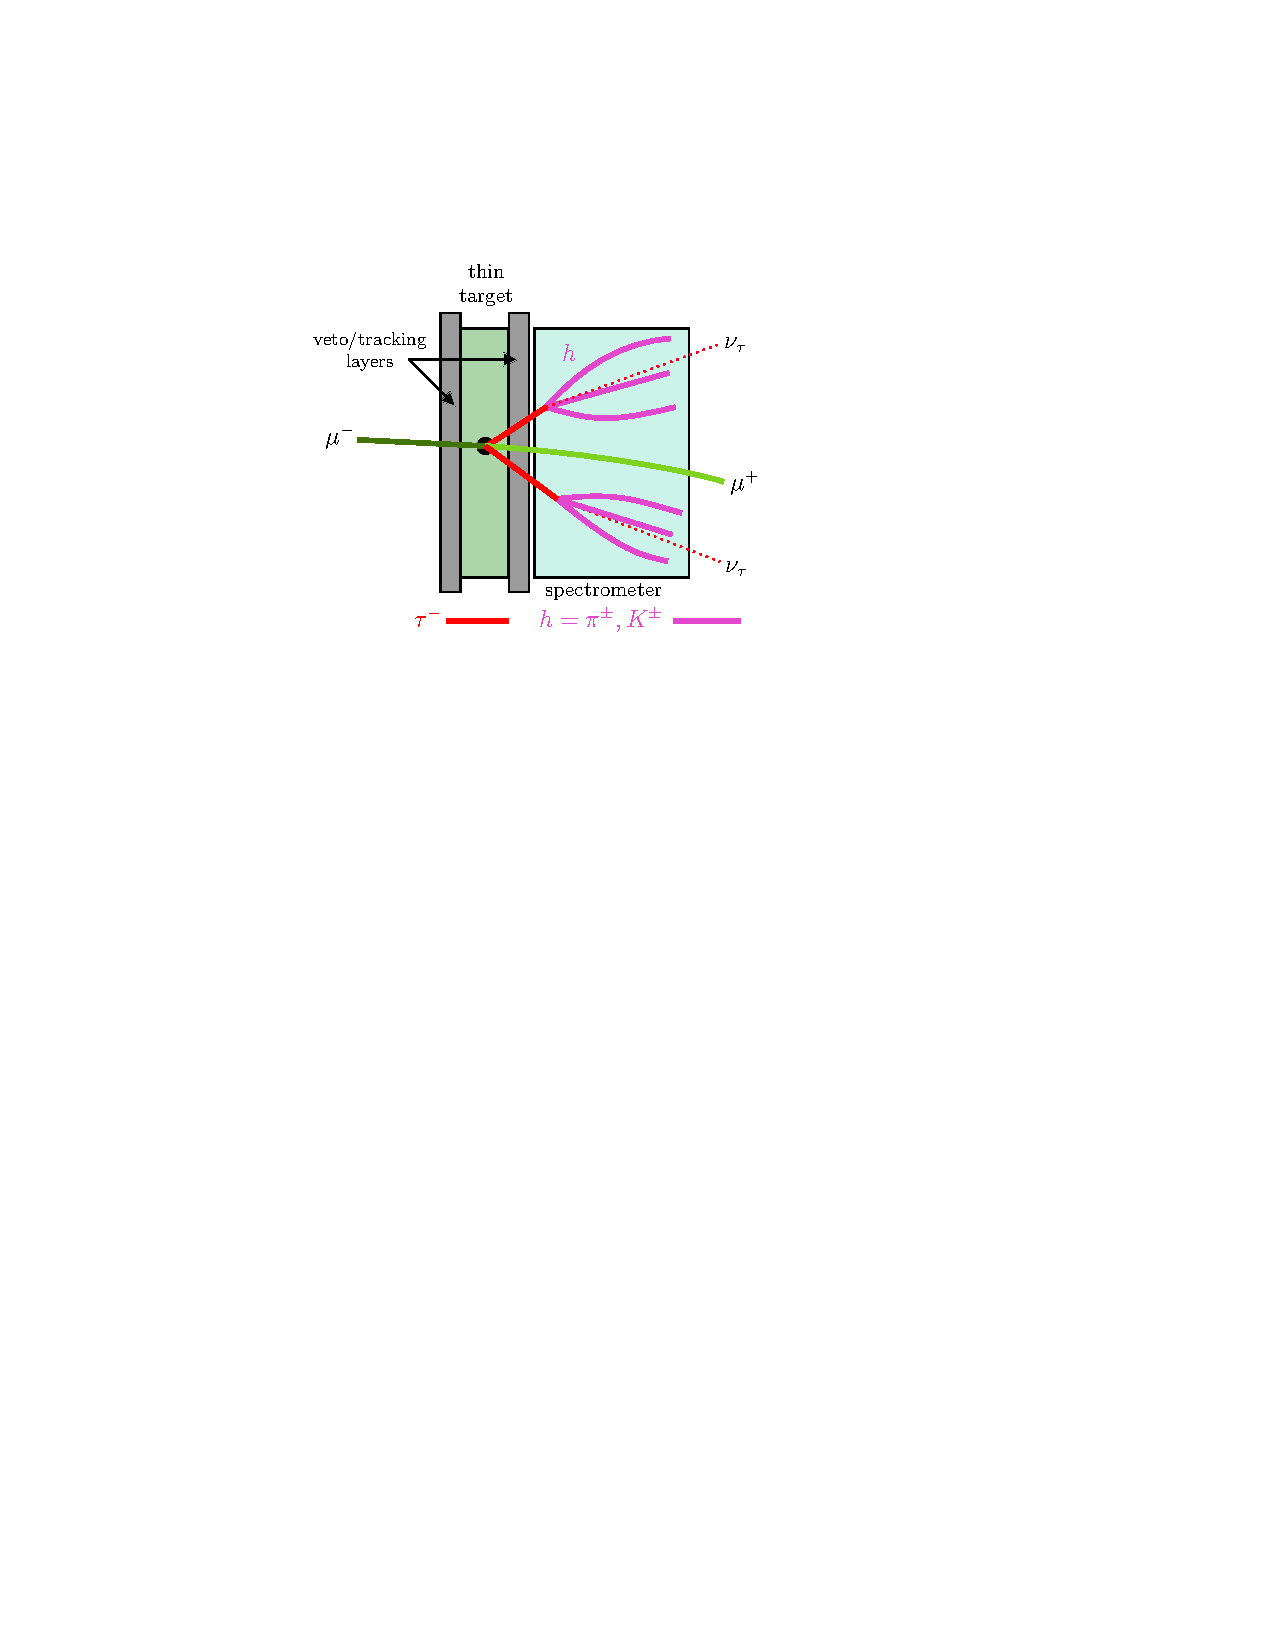
\includegraphics[width=0.5\linewidth]{figures/chapter5/spectrometer.pdf}
    \caption{A schematic representation of the fixed-target muon beam set up described in the text.}
    \label{fig:spectrometer}
\end{figure}

For concreteness, we consider a thin target composed of a $2~{\rm cm}$-thick lead plate, placed in between two veto or tracking layers and directly in front of a spectrometer. Interleaving this target with additional tracking layers could further improve the physics sensitivity, although this may be difficult given the length of the target. In the following, we will assume that a $2~{\rm cm}$ track identification resolution is required for identification of the $\tau$, essentially requiring it to pass through the external tracking layers and decay in the spectrometer. On top of tracking capabilities and energy measurement, muon identification is essential to study the signal of our interest. We assume that $\mu^\pm$s can be disentangled from charged pions with nearly 100\% efficiency.

The intensity and energy of the muon beam considered here are unprecedented in current and near-future experiments, which should be considered when designing the experiment. For instance, a highly collimated muon beam could potentially damage the active detector. in this case, defocusing the beam would be advantageous before it hits the target. The experiment could also operate under a reduced beam intensity in a short, dedicated run. Additional effects will be related to interactions of an electron cloud surrounding the muon beam. Being less energetic than muons, these could be partially deflected away or shielded on their way to the detector. These and other detector requirements, e.g., cooling, must be analyzed in detail to assess the feasibility of such a detector. We leave this for future studies. 

\begin{center}
    {\it 2. Muon (Synchrotron) Ion Collider (MuSIC)}
\end{center}

For the detector apparatus at MuSIC, we will follow Ref.~\cite{Acosta:2021qpx}, which proposes that the electron beam at the EIC is eventually upgraded to a 1 TeV muon beam for the purpose of probing deep nuclear structure. If interest for such a detector grows, it is possible that it will be constructed at another facility, but this has limited impact on our discussion. We assume that the gold ion energy remains at $110~{\rm GeV}/{\rm nucleon}$, which corresponds to a COM energy of $660~{\rm GeV}/{\rm nucleon}$, and a muon energy of $E = 20~{\rm TeV}$ in the rest frame of the gold ion. We will additionally assume a five-year integrated luminosity of ${\cal L} = 400/A~{\rm fb}^{-1} \approx 2~{\rm fb}^{-1}$ for gold. 

While the COM energy of a TeV muon-ion collider such as MuSIC is tantalizing, this comes with a cost: very low deflection angles. The situation is described more fully in  Section \ref{sec:phi_eta}; almost all particles (at least in the peripheral production process we are concerned with) have pseudorapidity $|\eta| > 4$. Hence, if the geometry of the detector is identical to that at the EIC (which has a pseudo-rapidity range $|\eta| < 3.5$), any hope of detecting particles produced in this way will be dashed. However, we anticipate that an experiment such as MuSIC would require a higher pseudo-rapidity range for the simple fact that TeV muons have a much higher inertia than $18~{\rm GeV}$ electrons, and thus will have lower deflection angles. In particular, we note that per the specifications of the ePIC collaboration (previously ECCE), the ion side of the EIC will currently be instrumented for tracking up to $4 < \eta < 6$ with the B0 spectrometer \cite{Adkins:2022jfp} for the purpose of identifying high-energy protons. We assume that a similar instrumentation can be added on the muon-side of interaction point, so that $|\eta| < 6$ can be achieved. While this will still not capture the majority of the MeV-scale particles MuSIC (see Fig.~\ref{fig:pseudorapidity_IQR}) it is sufficient for MuSIC to be sensitive to GeV-scale particles produced in peripheral interactions.


\subsection{Signal and Background}\label{MuSIC_MuBeD_ALP_BG}


\begin{center}
    {\it 1. Muon Beam Dump (MuBeD)}
\end{center}

The number of ALPs produced from the collision of a muon beam and a lead target of thickness $L_{\rm tar}$ which land inside the detector is given by \cite{Bjorken:2009mm,Cesarotti:2023sje}
\begin{align}
    \frac{dN}{dE_k\,dz} = \frac{N_\mu \rho_{\rm tar}}{M_{\rm tar}}\int_{E_k}^{E_0}{\frac{dE'}{E'}\int_0^{L_{\rm tar}} d\ell\,I(E'; E, \rho_{\rm tar}\ell/X_0)\times E_0\frac{d\sigma}{dE_k'}\frac{dP(z-\ell)}{dz}}
\end{align}
where $E$ is the incident energy, $N_\mu$ is the number of muons on target, $\rho_{\rm tar}$ and $M_{\rm tar}$ are the density and atomic mass of the material, $L_{\rm tar}$ is the length of the target, $X_0$ is the radiation length of the target, $P(z)$ is the probability the ALP decays a distance $z$ from where it is produced, and $I(E'; E, t)$ is a function which parametrizes radiative loss of the muon beam energy as it moves through the material. We specialize to the thin-target scenario, for which we can ignore energy loss of the muon beam as it moves through the material; e.g. $I(E'; E, \rho\ell/X_0) = \delta(E' - E)$. For the probability that the ALP decays a distance $z$ from where it is produced, we have
\begin{align}
    P(z) &= \Theta(z) \left(1-e^{-\frac{z}{\gamma c \tau_a}}\right)
\end{align}
where $\tau_a$ is the lifetime of the ALP and $\gamma$ its boost. Under the assumption that the ALP decays promptly (which we find is reasonable assumption for the masses and parameters probed), we have 
\begin{align}
    \frac{dN}{dE_k\,dz} &= \frac{N_\mu \rho_{\rm tar}}{M_{\rm tar}}\int_0^{L_{\rm tar}} d\ell\frac{d\sigma}{dE_k}\delta(z - \ell)\nonumber \\
    \implies N &= \frac{N_\mu \rho L_{\rm tar}}{M}\sigma
\end{align}
where we have used $P'(z) \approx \delta(z-\ell)$ for $\gamma c\tau_a \ll z$. This gives an effective integrated luminosity of ${\cal L}_{\rm eff.} = N_\mu (\rho_{\rm tar} L_{\rm tar}/M_{\rm tar})\approx (6.6\times 10^{-17}~{\rm fb}^{-1}) N_\mu$. Even for $N_\mu = 10^{16}$, this luminosity allows MuBeD to compete with the results from the EIC in the previous section, as well as the results from MuSIC (which is assumed to have a similar luminosity to the EIC). 

Like with the EIC, we will focus on the purely flavor-violating signal from $a \rightarrow \mu^+\tau^-$, which corresponds to half of all decay events. We assume that the $\mu^+$ can be identified with $100\%$ efficiency, and we veto on identification of a $\mu^-$ in the final state to ensure a purely LFV final state. We expect the final-state muon can also be vetoed with 100\% efficiency, since the detector can be instrumented directly in front of the muon beam (in contrast to the EIC, which has the possibility of losing the incident electron down the beam pipe). This alone should remove all SM background.\footnote{Given that the muon can also decay to an  electron and two neutrinos, it may be necessary to veto on identification of an electron in the final-state as well, but this does not affect our signal.} We also require identification of both $\tau^-$ in the final-state. We expect that the efficiency for this process can be relatively high if one combines charged tracks with hadronic final states in the spectrometer. In particular, we assume that all three-prong $\tau$s with a track length $>2~{\rm cm}$ can be resolved. To enforce the $2~{\rm cm}$ track-length requirement, we estimate the energy distributions of both $\tau^-$ then compute those fraction of $\tau^-$ for which $(E_\tau/m_\tau) c \tau_\tau > 2~{\rm cm}$, where $\tau_\tau$ is the rest-frame lifetime of the $\tau$. Labeling the $\tau$ converted from the muon $\tau_1$ and the $\tau$ which is a decay product of the ALP $\tau_2$, we can estimate the fraction of each $\tau$ that we detect. In particular, if the $\tau$ has Lorentz boost distribution $\rho_\gamma(\gamma_\tau)$, we define the $\tau$ detection efficiency as 
\begin{align}
    \epsilon_\tau &= {\cal B}(\tau \rightarrow \textrm{3-prong})\int_{(2{\rm cm})/c\tau_\tau}^{\infty} d\gamma_\tau\,\rho_\gamma(\gamma_\tau)
\end{align}
For $\tau_1$, we use the technique described in Section {\ref{sec:l_kin}} to compute its final-state boost distribution under the assumption that the photon transfer momentum is small, finding $\epsilon_\tau^{(1)} \approx 0.03\%-3\%$ over the range of masses considered. For $\tau_2$, we assume the ALP decays promptly, and the $\tau_2$ carries half of its energy $E_k/2$ away ($\gamma_\tau = E_k/(2m_\tau)$), finding $\epsilon_\tau^{(2)} \approx  5\%$ over the range of masses considered.



\begin{center}
    {\it 2. Muon (Synchrotron) Ion Collider (MuSIC)}
\end{center}

Given the similarities between MuSIC and the EIC, we will perform the same analysis as in Section \ref{sec:EIC_ALP}, but assuming we can detect decaying ALPs with $|\eta| < 6$. In particular, we will leverage the LFV final-state of the process $\mu^-A_Z \rightarrow \tau^- A_Z (a\rightarrow \mu^+\tau^-)$ by identifying the $\mu^+$ and a $\tau^-$. Like before, the leading background will be from ditau production (Fig.~\ref{fig:ditau_background}). Referring again to the cross-sections computed for ditau production from muons on rock \cite{Bulmahn:2008fa}, we estimate the cross-section for this at MuSIC (with $E = 20~{\rm TeV}$) is $\sigma_{\rm b.g.} \approx 10^5~{\rm pb}$. We will once again take the muon loss rate to be $10^{-2}$ and the rate of muon misidentification as an anti-muon to be $10^{-3}$. For direct comparison with the EIC, we will assume $\tau$ efficiencies of $\epsilon_\tau = 1\%$ and $\epsilon_\tau = 10\%$.
\begin{figure}[t!]
    \centering
    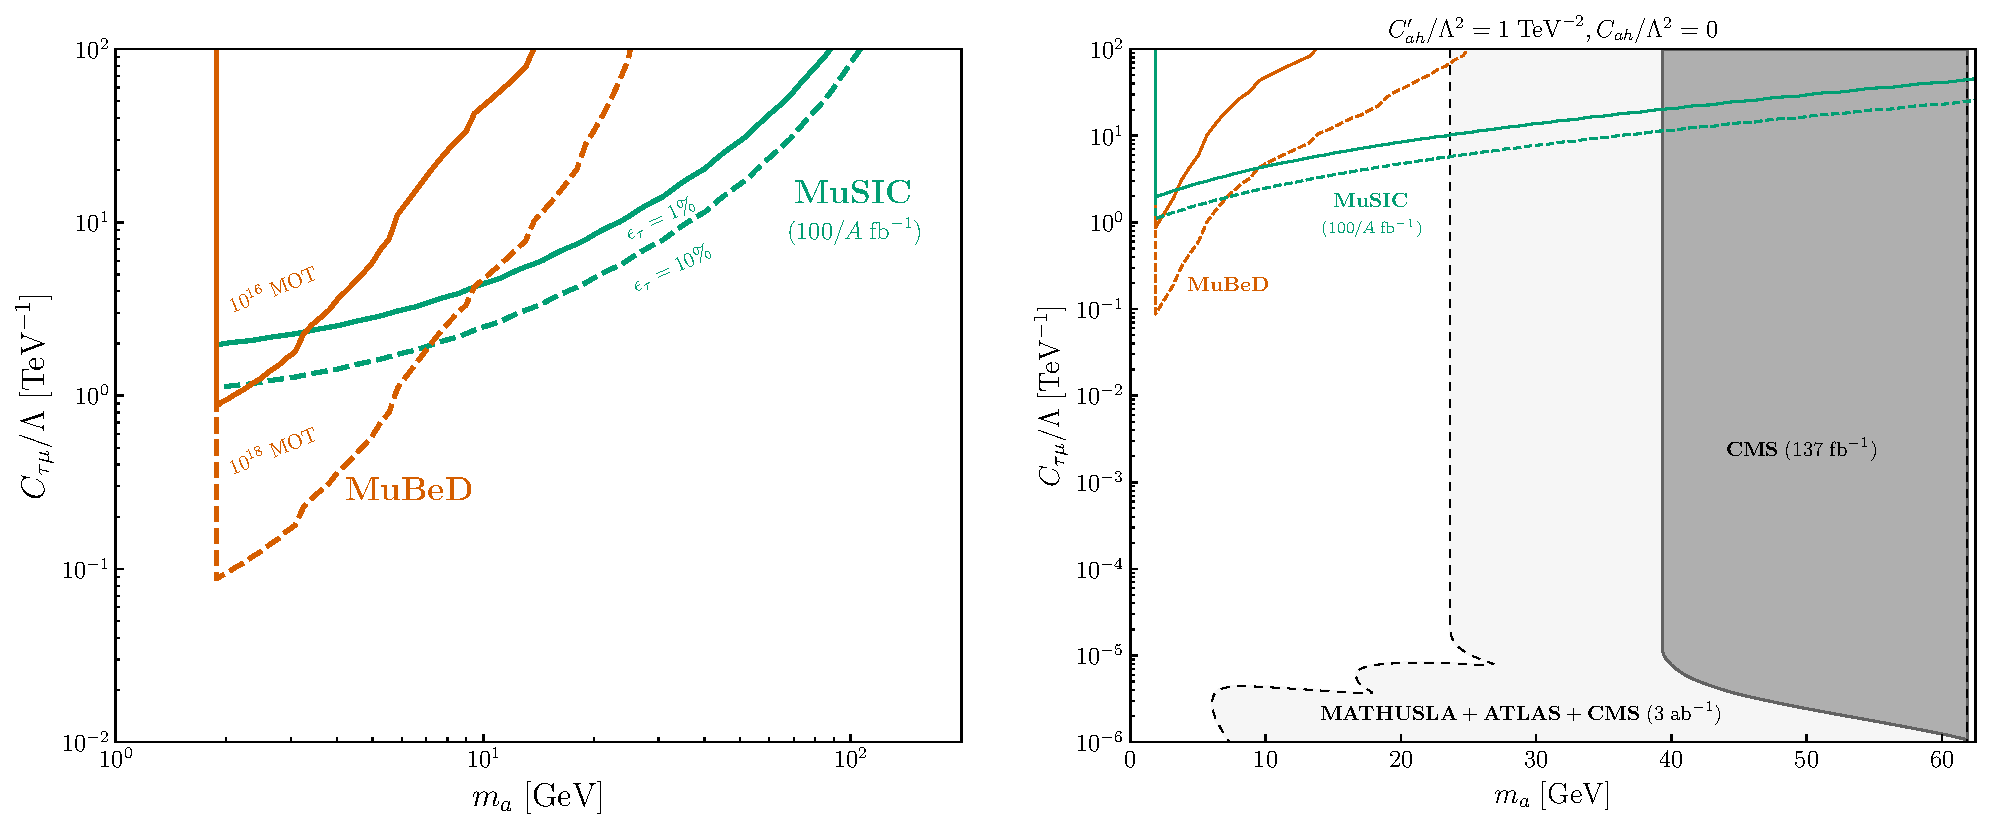
\includegraphics[width=\linewidth]{figures/chapter5/MuSIC_MuBeD_ALP_limits.pdf}
    \caption[Projected constraints on LFV ALPs at the MuBeD and MuSIC.]{(Left) limits on the LFV coupling $C_{\tau\mu}/\Lambda$ from MuBeD assuming $N_\mu = 10^{16}$ (orange, solid) and $N_\mu = 10^{18}$ (orange, dashed), and from MuSIC assuming a $\tau$ efficiency of $\epsilon_\tau = 1\%$ (green, solid) and $\epsilon_\tau = 10\%$ (green, dashed). (Right) the same limits in the larger context of the LHC Higgs decay limits from the last section, assuming $C_{ah}'/\Lambda^2 = 1~{\rm TeV}^{-2}$ and $C_{ah}/\Lambda^2 = 0~{\rm TeV}^{-2}$. These limits are recast to the scenario in which $C_{\tau\mu}$ is the only non-zero coupling of the ALP.}
    \label{fig:EIC_ALP_limits}
\end{figure}
\subsection{Combined Limits}\label{sec:MuBeD_MuSIC_ALP_limits}
We are now equipped to place $95\%$ exclusion limits on the $C_{\tau\mu}$ couplings from each of these experiments. Beginning with MuBeD, the zero-background signal entails that the coupling $C_{\mu\tau}$ is excluded at the $95\%$ C.L. by
\begin{align}
    \frac{C_{\tau\mu}}{\Lambda}~{({\rm MuBeD})} \leq \sqrt{\frac{3.09}{\epsilon_\tau^{(1)}\epsilon_\tau^{(2)}\hat{\sigma}{\cal L}_{\rm eff.}}}~{\rm TeV}^{-1} \sim \sqrt{\frac{6\times 10^{15}~{\rm pb}}{N_\mu \hat{\sigma}}}~{\rm TeV}^{-1}
\end{align}
where $\hat{\sigma}$ is the production cross-section normalized by $(C_{\tau\mu}/\Lambda)^2$. 

For MuSIC, the signal is not zero-background. Rather, the analysis in the previous section indicates there will be approximately $N_{\rm b.g.} = 180000\epsilon_\tau$ background events. To place $95\%$ C.L. ($2\sigma$) limits on the coupling $C_{\tau e}/\Lambda$, we find the value of $C_{\tau e}/\Lambda$ for which the number of expected signal events is $N_{\rm sig} = 2\sqrt{N_{\rm b.g.}} \approx 850\sqrt{\epsilon_\tau}$. Hence, the MuSIC bounds are given by
\begin{align}
    \frac{C_{\tau\mu}}{\Lambda}~{({\rm MuSIC})}\leq \sqrt{\frac{850}{\sqrt{\epsilon_\tau}\hat{\sigma}{\cal L}}}~{\rm TeV}^{-1} \sim\sqrt{\frac{1.7~{\rm pb}}{\sqrt{\epsilon_\tau} \hat{\sigma}}}~{\rm TeV}^{-1}
\end{align}
One downside of MuSIC (and the EIC) for detection through this production process is that there is not much room for improvement. Their luminosity is fundamentally limited by the ability to focus the lepton and ion beams, and the detector geometry is inopportune for capturing particles which are produced with high pseudo-rapidity.
\begin{figure}[t!]
    \centering
    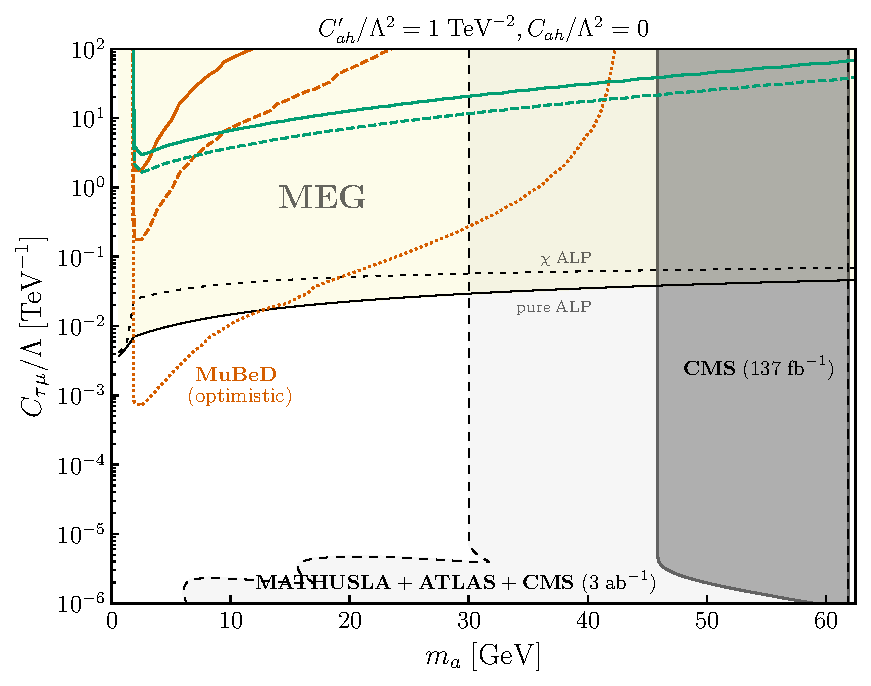
\includegraphics[width=0.6\linewidth]{figures/chapter5/MuBeD_optimistic.pdf}
    \caption[Optimistic projected constraints on LFV ALPs at MuBeD.]{Limits on $C_{\tau\ell}/\Lambda$ for democratic ALP-lepton couplings, assuming the most optimistic scenario for a muon beam dump experiment (described in the text). The leading constraint for the democratic scenario from LFV lepton decays comes from the MEG experiment due to the process $\mu\stackrel{\tau}{\longrightarrow}e\gamma$, which is enhanced by the $\tau$ mass at both LFV vertices.}
    \label{fig:MuBeD_optimistic}
\end{figure}
For MuBeD, on the other hand, we have made somewhat modest assumptions. While we have assumed an instrumented target of length $L_{\rm tar} = 2~{\rm cm}$, it is not difficult to imagine a much thicker target, such as the proposed $2~{\rm m}$ thick FASER$\nu$2 detector at the Forward Physics Facility at CERN \cite{FPFWorkingGroups:2025rsc}. This would also allow for finer $\tau$ track resolution, and hence a better $\tau$ detection efficiency.

In Fig~\ref{fig:MuBeD_optimistic}, we plot the {\it most} optimistic case for MuBeD which is still experimentally reasonable: $N_\mu = 10^{20}$, $L_{\rm tar} = 2~{\rm m}$, and a $\tau$ track resolution of $2~{\rm mm}$. In particular, such a $\tau$ track resolution could be achieved if the $2~{\rm m}$ lead target is interleaved with trackers or emulsion detectors, again like FASER$\nu$2. Rather than focusing on a singular off-diagonal coupling, here we focus on the ``democratic'' coupling scenario, for which all of the ALP-lepton couplings are the same. While the democratic scenario is already excluded beyond the reach of the EIC and MuSIC by LFV lepton decays, we see that the most optimistic scenario for MuBeD is competitive with these constraints. 

\subsection{Explanation to $(g-2)_\mu$ Anomaly}\label{sec:MuBeD_MuSIC_g_2}

Here, we perform a similar analysis to the analysis performed in Section~{\ref{sec:EIC_ALP_g_2}} for probing explanations to the electron $g-2$ at the EIC. In particular, we will explore the sensitivity of MuSIC and MuBeD to PV ALP explanations to the muon $g-2$ anomaly. One notable difference is that there is only {\it one} muon $g-2$ anomaly, and it is a {\it positive} anomaly. For ALPs, this corresponds to PV angles $\Theta\gtrsim \pi/4$.
\begin{figure}[t!]
    \centering
    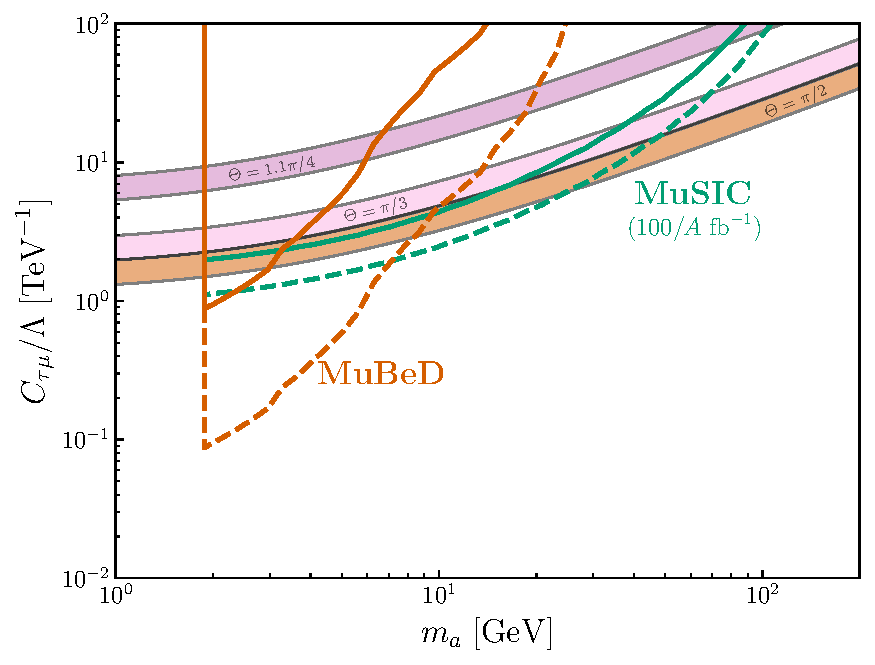
\includegraphics[width=0.6\linewidth]{figures/chapter5/MuSIC_MuBeD_ALP_muon_g_2.pdf}
    \caption[Projected constraints on LFV ALPs at the MuBeD and MuSIC, alongside LFV ALP explanations to the muon $g-2$ anomaly.]{Expected limits on $C_{\tau \mu}/\Lambda$ from MuBeD and MuSIC, alongside explanations for the muon $g-2$ anomaly for different PV angles $\Theta$.}
    \label{fig:MuSIC_MuBeD_g_2}
\end{figure}
PV ALP explanations to the muon $g-2$ anomaly were already explored in Section \ref{sec:g-2_explanation}, and the resulting couplings $C_{\tau\mu}$ are notably within reach of the limits found for MuBeD and MuSIC in the previous Section. We plot these constraints alongside explanations to the muon $g-2$ anomaly for three representative angles in Fig.~\ref{fig:MuSIC_MuBeD_g_2}. In this case, for all angles that contribute the right sign to the anomaly, there is a range of masses $m_a$ for which both MuSIC and MuBeD probe solutions to the anomaly. While MuBeD requires less statistics to probe solutions at smaller masses, MuSIC has the advantage at probing larger-mass solutions to the $g-2$ anomaly.
\begin{figure}[t!]
    \centering
    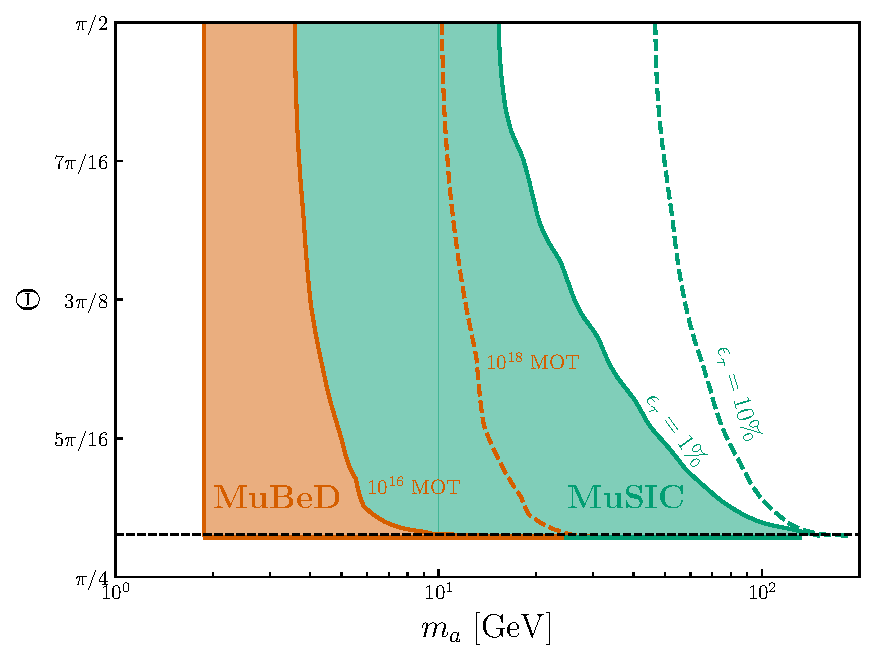
\includegraphics[width=0.6\linewidth]{figures/chapter5/MuSIC_MuBeD_g_2_probe.pdf}
    \caption[Region in the $m_a$-$\Theta$ plane for which MuBeD and MuSIC probe an LFV ALP explanation to the muon $g-2$ anomaly.]{The region in the $m_a$-$\Theta$ plane for which MuBeD and MuSIC probe an LFV ALP explanation to the muon $g-2$ anomaly.}
    \label{fig:MuSIC_MuBeD_g_2_region}
\end{figure}
In Fig.~\ref{fig:MuSIC_MuBeD_g_2_region}, we plot the region in the $\Theta$-$m_a$ parameter-space for which MuBeD and MuSIC probe solutions to the muon $g-2$ anomaly. This reemphasizes the point that while both experiments can probe solutions for any permissable angle $\Theta$, MuSIC has a wider mass-reach. 

Although we have presented these results for an ALP, the fact that the explanation requires $\Theta > \pi/4$ is in-line with the understanding that scalars, not pseudoscalars, contribute the correct sign to account for the $(g-2)_\mu$ anomaly. Nonetheless, as we have explored in previous chapters, the notions of ``scalar'' vs. ``pseudo-scalar'' are less concrete for flavor off-diagonal interactions, so it is reasonable to consider an ALP with $\Theta > \pi/4$.
